% ------------------------------------------------------------------------------
% Formatvorlage für Abschlussarbeiten an der Hochschule Ulm, Prof. Dr. Rr. von Schwerin
% ------------------------------------------------------------------------------
%   
%   Original erstellt von Stefan Macke, 24.04.2009
%   http://blog.stefan-macke.de
% Dokumentenkopf ---------------------------------------------------------------
%   Diese Vorlage basiert auf "scrreprt" aus dem koma-script.
% ------------------------------------------------------------------------------
\documentclass[
    12pt, % Schriftgröße
    DIV10,
%    ngerman, % für Umlaute, Silbentrennung etc.
    american,
    a4paper, % Papierformat
    oneside, % einseitiges Dokument
    titlepage, % es wird eine Titelseite verwendet
    parskip=half, % Abstand zwischen Absätzen (halbe Zeile)
    headings=normal, % Größe der Überschriften verkleinern
    listof=totoc, % Verzeichnisse im Inhaltsverzeichnis aufführen
    bibliography=totoc, % Literaturverzeichnis im Inhaltsverzeichnis aufführen
    index=totoc, % Index im Inhaltsverzeichnis aufführen
    captions=tableheading, % Beschriftung von Tabellen unterhalb ausgeben
    final % Status des Dokuments (final/draft)
]{scrreprt}
%
% Verweis auf Abbildungsverzeichnis im Text ermöglichen
%
\BeforeStartingTOC[lof]{\label{listoffigures}}

% Kodierung als erstes, daher in der Hauptdatei, nicht in Packages (s.u.)
%
% Anpassung an Landessprache ---------------------------------------------------
%\usepackage[ngerman]{babel}
\usepackage[USenglish]{babel}

% Umlaute ----------------------------------------------------------------------
%   Umlaute/Sonderzeichen wie äüöß direkt im Quelltext verwenden (CodePage).
%   Erlaubt automatische Trennung von Worten mit Umlauten.
% ------------------------------------------------------------------------------
\usepackage[utf8]{inputenc}
\usepackage[T1]{fontenc}
\usepackage{textcomp} % Euro-Zeichen etc.
%
% Schalter für print oder PDF definieren
%
% https://golatex.de/eigene-schalter-fuer-verschiedene-varianten-t7130.html
\newif\ifprint
%\printtrue  % für die Druckversion
\printfalse  % für die PDF-Version

% Meta-Informationen -----------------------------------------------------------
%   Informationen über das Dokument, wie z.B. Titel, Autor, Matrikelnr. etc
%   werden in der Datei Meta.tex definiert und können danach global
%   verwendet werden.
% ------------------------------------------------------------------------------
% Meta-Informationen -----------------------------------------------------------
%   Definition von globalen Parametern, die im gesamten Dokument verwendet
%   werden können (z.B auf dem Deckblatt etc.).
%
%   ACHTUNG: Wenn die Texte Umlaute oder ein Esszet enthalten, muss der folgende
%            Befehl bereits an dieser Stelle aktiviert werden:
%            \usepackage[utf8]{inputenc}
% ------------------------------------------------------------------------------
%
% Bitte anpassen: 
%   Abschlussarbeit --> Bachelorarbeit oder Masterarbeit
%
%
\newcommand{\titel}{Data Science Project}
\newcommand{\untertitel}{Prediction of Soccer Results}
\newcommand{\art}{Technical Report}
\newcommand{\verfasser}{Martin Schmid, Sergej Dechant, Lisa Boos, Khaled Jalloulli}
\newcommand{\matrikelnr}{1234567}
\newcommand{\studiengang}{Master - Information Systems}
\newcommand{\erstgutachter}{Prof.~Dr.~Volker Herbort}
\newcommand{\zweitgutachter}{Prof.~Dr.~Markus Goldstein}
\newcommand{\abgabedatum}{32. Monat 9999}
\newcommand{\jahr}{2019}
\newcommand{\ort}{Ulm}
\newcommand{\logo}{HochschulLogo_de.jpg}


% benötigte Packages -----------------------------------------------------------
%   LaTeX-Packages, die benötigt werden, sind in die Datei Packages.tex
%   "ausgelagert", um diese Vorlage möglichst übersichtlich zu halten.
% ------------------------------------------------------------------------------
% Anpassung des Seitenlayouts --------------------------------------------------
%   siehe Seitenstil.tex
% ------------------------------------------------------------------------------
%\usepackage[
%    automark, % Kapitelangaben in Kopfzeile automatisch erstellen
%    headsepline, % Trennlinie unter Kopfzeile
%    ilines % Trennlinie linksbündig ausrichten
%]{scrpage2}
%
% Nutzung des aktuelleren Pakets
\usepackage[
    automark, % Kapitelangaben in Kopfzeile automatisch erstellen
    headsepline, % Trennlinie unter Kopfzeile
    ilines % Trennlinie linksbündig ausrichten
]{scrlayer-scrpage}
% zur Vermeidung von float-warnings
\usepackage{scrhack}
% für bessere Umbruchpunkte
% siehe: https://texfragen.de/overfull_hbox
\usepackage{microtype}

% Moderneres Backend für das Literaturverzeichnis
% Quelle: https://golatex.de/vorlage-fuer-abschlussarbeiten-htwk-leipzig-t18498.html
%
\usepackage[
    backend=biber,
%    style=numeric-comp,  % entspricht dem Stil der AMS
%    style=authoryear, % entspricht dem Harvard-Stil
    style=ieee, % entspricht dem IEEE-Stil
%    natbib,
    sorting=nyt,
    defernumbers=true,
    backref=true,
    giveninits=true, % Initialen statt vollständige Vornamen
    uniquename=init,
    doi=false,
    isbn=false
]{biblatex}
% Familienname in Käpitälchen im Literaturverzeichnis
\renewcommand*{\mkbibnamefamily}[1]{\textsc{#1}}
%\renewcommand*{\mkbibnamefirst}[1]{#1\addcomma}
%\renewcommand*{\mkbibnameprefix}[1]{\textsc{#1}}
\addbibresource{Bibtex/sources.bib}
\setlength{\bibitemsep}{0.5\baselineskip}
% siehe: https://tex.stackexchange.com/questions/39285/whats-the-advantage-of-using-csquotes-over-using-an-editors-auto-replacement-f
\usepackage[babel, german=quotes]{csquotes}
\renewcommand{\mkcitation}[1]{#1}

% Schrift ----------------------------------------------------------------------
\usepackage{lmodern} % bessere Fonts
\usepackage{relsize} % Schriftgröße relativ festlegen

% Grafiken ---------------------------------------------------------------------
% Einbinden von JPG-Grafiken ermöglichen
\usepackage[dvips,final]{graphicx}
% hier liegen die Bilder des Dokuments
\graphicspath{{Bilder/}}

% Befehle aus AMSTeX für mathematische Symbole z.B. \boldsymbol \mathbb --------
\usepackage{amsmath,amsfonts}

% für Index-Ausgabe mit \printindex --------------------------------------------
\usepackage{makeidx}

% Einfache Definition der Zeilenabstände und Seitenränder etc. -----------------
\usepackage{setspace}
\usepackage{geometry}

% zum Umfließen von Bildern ----------------------------------------------------
\usepackage{floatflt}
% Zum Erzwingen der Platzierung von Tabellen und Abbildungen mitels [H] --------
\usepackage{float}

\usepackage[dvipsnames]{xcolor}        %  erm"oglicht Benutzung von Farbe durch Namensgebung 

% fortlaufendes Durchnummerieren der Fußnoten ----------------------------------
\usepackage{chngcntr}

% für lange Tabellen -----------------------------------------------------------
\usepackage{booktabs}
% für lange Tabellen -----------------------------------------------------------
\usepackage{longtable}
\usepackage{array}
\usepackage{ragged2e}
\usepackage{lscape}

% Spaltendefinition rechtsbündig mit definierter Breite ------------------------
\newcolumntype{w}[1]{>{\raggedleft\hspace{0pt}}p{#1}}

% Formatierung von Listen ändern -----------------------------------------------
\usepackage{paralist}

% bei der Definition eigener Befehle benötigt
\usepackage{ifthen}

% definiert u.a. die Befehle \todo, \missingfigure und \listoftodos
% siehe: https://mirror.hmc.edu/ctan/macros/latex/contrib/todonotes/todonotes.pdf
\usepackage{todonotes}

% sorgt dafür, dass Leerzeichen hinter parameterlosen Makros nicht als Makroendezeichen interpretiert werden
\usepackage{xspace}

% stellt zusätzliche Symbole bereit (z.B. \Square == Checkbox)
% siehe: http://texdoc.net/texmf-dist/doc/latex/wasysym/wasysym.pdf
\usepackage{wasysym}

% flexible Verweise
% siehe: https://ctan.org/pkg/varioref
\usepackage{varioref}

% zum Einbinden von Programmcode -----------------------------------------------
\usepackage{listings}
%
\definecolor{hellgrau}{rgb}{0.95,0.95,0.95}
\definecolor{dkgreen}{rgb}{0,0.6,0}
\definecolor{hellgruen}{rgb}{.7,1,.7}
\definecolor{gray}{rgb}{0.5,0.5,0.5}
\definecolor{mauve}{rgb}{0.58,0,0.82}
\definecolor{orange1}{RGB}{255,153,102}
\definecolor{hellgelb}{RGB}{255,255,204}
\definecolor{hellgrau1}{RGB}{204,204,204}
\definecolor{LightGray}{gray}{0.9} % new color for background of listing
%
\lstset{ %
  language=Python,                % the language of the code
  %basicstyle=\small, % print whole listing small
  %basicstyle=\footnotesize,       % the size of the fonts that are used for the code
  basicstyle=\ttfamily\footnotesize,
  numbers=left,                   % where to put the line-numbers
  numberstyle=\tiny\color{gray},  % the style that is used for the line-numbers
  stepnumber=1,                   % the step between two line-numbers. If it's 1, each line 
                                  % will be numbered
  numbersep=5pt,                  % how far the line-numbers are from the code
  backgroundcolor=\color{LightGray},  % choose the background color. You must add \usepackage{color}
  showspaces=false,               % show spaces adding particular underscores
  showstringspaces=false,         % underline spaces within strings
  showtabs=false,                 % show tabs within strings adding particular underscores
  frame=single,                   % adds a frame around the code
  rulecolor=\color{black},        % if not set, the frame-color may be changed on line-breaks within not-black text (e.g. commens (green here))
  tabsize=4,                      % sets default tabsize to 4 spaces (in accordance with Python)
  captionpos=b,                   % sets the caption-position to bottom
  breaklines=true,                % sets automatic line breaking
  breakatwhitespace=false,        % sets if automatic breaks should only happen at whitespace
  title=\lstname,                 % show the filename of files included with \lstinputlisting;
                                  % also try caption instead of title
  keywordstyle=\color{blue},      % keyword style
  commentstyle=\color{dkgreen},   % comment style
  stringstyle=\color{mauve},      % string literal style
  escapeinside={\%*}{*)},         % if you want to add LaTeX within your code
  morekeywords={*,...}            % if you want to add more keywords to the set
}

% Umlaute in Listings (Kommentaren) verarbeiten
\lstset{
  literate={ö}{{\"o}}1
           {ä}{{\"a}}1
           {ü}{{\"u}}1
           {Ö}{{\"O}}1
           {Ä}{{\"A}}1
           {Ü}{{\"U}}1
           {ß}{{\"s}}1
}

% URL verlinken, lange URLs umbrechen etc. -------------------------------------
\usepackage{url}

% wichtig für korrekte Zitierweise ---------------------------------------------
% ersetzt durch biblatex + biber
%\usepackage[square]{natbib}

% PDF-Optionen -----------------------------------------------------------------
%
\usepackage[
    bookmarks,
    bookmarksopen=true,
    colorlinks=true,
%    backref, -- nicht mit biblatex vereinbar; dortige Option verwenden!
    plainpages=false, % zur korrekten Erstellung der Bookmarks
    pdfpagelabels, % zur korrekten Erstellung der Bookmarks
    hypertexnames=true, % zur korrekten Erstellung der Bookmarks
    linktocpage % Seitenzahlen anstatt Text im Inhaltsverzeichnis verlinken
]{hyperref}
% 
% Nutzung des Schalters für Druck/PDF (Datei Abschlussarbeit.tex Zeilen 46 -- 48)
%
\ifprint 
% alles schwarz
\hypersetup{
    linkcolor=black,
    anchorcolor=black,% Ankertext
    citecolor=black, % Verweise auf Literaturverzeichniseinträge im Text
    filecolor=black, % Verknüpfungen, die lokale Dateien öffnen
    menucolor=black, % Acrobat-Menüpunkte
    urlcolor=black % Verweise auf Webseiten
    }
\else
% farbig
\hypersetup{
    linkcolor=CadetBlue,
    anchorcolor=black,% Ankertext
    citecolor=blue, % Verweise auf Literaturverzeichniseinträge im Text
    filecolor=magenta, % Verknüpfungen, die lokale Dateien öffnen
    menucolor=red, % Acrobat-Menüpunkte
    urlcolor=ForestGreen % Verweise auf Webseiten
	}
\fi
%
% Meta-Informationen
%
\hypersetup{
    pdftitle={\titel \untertitel},
    pdfauthor={\verfasser},
    pdfcreator={\verfasser},
    pdfsubject={\titel \untertitel},
    pdfkeywords={\titel \untertitel},
}

% ---- Paket für Abkürzungen, Symbole und Erklärungen ---
% Einführung siehe: https://www.dante.de/events/dante2015/Programm/vortraege/vortrage-partosch.pdf
\usepackage[%
toc, % ins Inhaltsverzeichnis übernehmen
nonumberlist, % keine Seitenzahlen
symbols, % ermöglichst Symbole+Symbolverzeichnis
acronym % ermoeglicht Abkuerzungen+Abkuerzungsverz.
]{glossaries} % ermoeglicht Glossar, ...
\renewcommand*{\glspostdescription}{}
%
% ---- Paket für Bilder
%
\usepackage{tikz}
\usetikzlibrary{positioning} % für Beispiel mit Listing



% Kopf- und Fußzeilen, Seitenränder etc. ---------------------------------------
% Zeilenabstand 1,5 Zeilen -----------------------------------------------------
\onehalfspacing

% Seitenränder -----------------------------------------------------------------
\setlength{\topskip}{\ht\strutbox} % behebt Warnung von geometry
%\geometry{paper=a4paper,left=35mm,right=35mm,top=30mm}
\geometry{
	includeheadfoot,
	top = 20mm,
	inner = 25mm,
	outer = 30mm, 
	bottom = 30mm,
	bindingoffset = 5mm,
	marginparwidth = 25mm
	}


% Kopf- und Fußzeilen ----------------------------------------------------------
\pagestyle{scrheadings}
% Kopf- und Fußzeile auch auf Kapitelanfangsseiten
%\renewcommand*{\chapterpagestyle}{scrheadings} 

% Schriftform der Kopfzeile
\renewcommand{\headfont}{\normalfont}

% Kopfzeile
\ohead{\textit{\headmark}}
\chead{}
\ihead{}
\setlength{\headheight}{21mm} % Höhe der Kopfzeile
% Kopfzeile über den Text hinaus verbreitern
% \setheadwidth[0pt]{textwithmarginpar} 
%\setheadsepline[text]{0.4pt} % Trennlinie unter Kopfzeile

% Fußzeile
%\ifoot{\copyright\ \verfasser, \jahr}
\ifoot{}
\cfoot{}
\ofoot{\pagemark}

% sonstige typographische Einstellungen ----------------------------------------

% erzeugt ein wenig mehr Platz hinter einem Punkt
\frenchspacing 

% Schusterjungen und Hurenkinder vermeiden
\clubpenalty = 10000
\widowpenalty = 10000 
\displaywidowpenalty = 10000

% Quellcode-Ausgabe formatieren
\lstset{numbers=left, numberstyle=\tiny, numbersep=5pt, breaklines=true}
\lstset{emph={square}, emphstyle=\color{red}, emph={[2]root,base}, emphstyle={[2]\color{blue}}}

% Fußnoten fortlaufend durchnummerieren
\counterwithout{footnote}{chapter}


% eigene Definitionen für Silbentrennung
% Trennvorschläge im Text werden mit \" angegeben
% untrennbare Wörter und Ausnahmen von der normalen Trennung können in dieser
% Datei mittels \hyphenation definiert werden
\hyphenchar\font=\string"7F
\hyphenation{Ge-schäfts-pro-zess}


% eigene LaTeX-Befehle
% Eigene Befehle und typographische Auszeichnungen für diese

% einfaches Wechseln der Schrift, z.B.: \changefont{cmss}{sbc}{n}
\newcommand{\changefont}[3]{\fontfamily{#1} \fontseries{#2} \fontshape{#3} \selectfont}

% Abkürzungen mit korrektem Leerraum 
\renewcommand{\dh}{\mbox{d.\,h.\ }} 
% Achtung: \dh existiert bereits für den isländischen Buchstaben Eth, was wohl eher nicht benötigt werden dürfte ...
\newcommand{\ua}{\mbox{u.\,a.\ }}
\newcommand{\zB}{\mbox{z.\,B.\ }}
\newcommand{\dahe}{\mbox{d.\,h.\ }}
\newcommand{\Vgl}{Vgl.\ }
\newcommand{\bzw}{bzw.\ }
\newcommand{\evtl}{evtl.\ }

% einfachere Referenzierung von Abbildungen und Tabellen
\newcommand{\abbildung}[1]{Abbildung~\vref{fig:#1}}
\newcommand{\tabelle}[1]{Tabelle~\vref{tab:#1}}
\newcommand{\listing}[1]{Listing~\vref{lst:#1}}

\newcommand{\bs}{$\backslash$}

% erzeugt ein Listenelement mit fetter Überschrift 
\newcommand{\itemd}[2]{\item{\textbf{#1}}\\{#2}}

% einige Befehle zum Zitieren --------------------------------------------------
\newcommand{\Zitat}[2][\empty]{\ifthenelse{\equal{#1}{\empty}}{\citep{#2}}{\citep[#1]{#2}}}

% zum Ausgeben von Autoren
\newcommand{\AutorName}[1]{\textsc{#1}}
\newcommand{\Autor}[1]{\AutorName{\citeauthor{#1}}}

% verschiedene Befehle um Wörter semantisch auszuzeichnen ----------------------
\newcommand{\NeuerBegriff}[1]{\textbf{#1}}
\newcommand{\Fachbegriff}[1]{\textit{#1}}

\newcommand{\Eingabe}[1]{\texttt{#1}}
\newcommand{\Code}[1]{\texttt{#1}}
\newcommand{\Datei}[1]{\texttt{#1}}
\newcommand{\Paket}[1]{\texttt{#1}}

\newcommand{\Software}[1]{\textsf{#1}}


% Abkürzungsverzeichnis --------------------------------------------------------
\makeglossaries
\loadglsentries{Inhalt/Glossar.tex}

% Das eigentliche Dokument -----------------------------------------------------
%   Der eigentliche Inhalt des Dokuments beginnt hier. Die einzelnen Seiten
%   und Kapitel werden in eigene Dateien ausgelagert und hier nur inkludiert.
% ------------------------------------------------------------------------------
\begin{document}
%\selectlanguage{ngerman}
\selectlanguage{american}
% auch subsubsection nummerieren
\setcounter{secnumdepth}{3}
\setcounter{tocdepth}{3}

% Seitennummerierung -----------------------------------------------------------
%   Die ersten beiden Seiten werden nicht nummeriert -> wir nehmen einen sonst
%   nicht verwendeten Stil, um hyperref sonst nicht verwendete "Seitennamen"
%   vorzugaukeln (Option: hypertexnames=true !)
%
%  siehe https://tex.stackexchange.com/questions/58941/hyperref-pagebackref-page-number-and-link-in-references-wrong/58962#58962
% ------------------------------------------------------------------------------
\pagenumbering{Alph}
% Deckblatt und Abstract ohne Seitenzahl
\ofoot{}
\begin{titlepage}
    \newcommand{\HRule}{\rule{\linewidth}{1.5mm}}
    \center{}
    \begin{figure}
        \centering
        
\includegraphics[width=0.5\textwidth]{../Bilder/th-ulm}\label{pic:Logo}
    \end{figure}

    \begin{center}
    \end{center}

    {\huge Masterproject}\\[0.4cm]
    \begin{center}
    \end{center}
    {\Large Prediction of Soccer Games }\\
    \vfill
    \begin{center}
        {Contributors:}\ \\
        \vspace{0.25\baselineskip}
        {\Large Lisa Boos, Sergej Dechant, Khaled Jalloulli, Martin Schmid}
    \end{center}
    \vfill
    \begin{center}
        {\large Expert: Prof.\ Dr.\ Volker Herbort}
    \end{center}
    \begin{center}
        {\large Expert: Prof.\ Dr.\ Markus Goldstein}
    \end{center}
    \vfill
    {\Large \today}

\end{titlepage}
\cleardoublepage
%\section*{Eigenständigkeitserklärung}
Diese Abschlussarbeit wurde von mir selbständig verfasst. Es wurden nur die angegebenen Quellen und Hilfsmittel verwendet. Alle wörtlichen und sinngemäßen Zitate sind in dieser Arbeit als solche kenntlich gemacht.\\[3em]
\parindent0mm
\vspace{2cm}
\ort, \abgabedatum \hspace{2cm}  Unterschrift: \begin{tikzpicture}[line width=1pt]\draw (2,0) -- (8,0);\end{tikzpicture}\\ % Selbständigkeitserklärung
%\cleardoublepage
%\section*{Zusammenfassung}
\label{sec:Zusammenfassung}
Diese Vorlage dient der Erstellung von Abschlussarbeiten mit \LaTeX.
Dabei werden einige Aspekte direkt angesprochen, während andere sich erst erschließen, indem man sich die Verzeichnis- und Dateistruktur sowie die Inhalte der eingebundenen Dateien ansieht. Aus den Kommentaren wird klar, was der jeweilige Zweck ist. Ansonsten hilft eine kurze Internetrecherche meist weiter.

Einige Kapitel, insbesondere diejenigen zu den Forschungsmethoden (\ref{cha:Forschungsmethoden}) und zum Zitieren
(\ref{cha:ZitateReferenzen}), sind jedoch auch dann zu beachten, wenn die Erstellung der Arbeit mit einem anderen
Textverarbeitungs- und Satzprogramm erfolgt. Dies gilt natürlich auch für Anhang \ref{anh:Anh-Anforderungen}!

Das Dokument zeigt, dass mit \LaTeX{} optisch äußerst hochwertige Dokumente erzeugt werden können, bei denen
sich das Programm außerdem noch automatisch um die Einhaltung weiterer Anforderungen kümmert.


\section*{Abstract}
\label{sec:Abstract}
This template shall help in writing a thesis using \LaTeX.
Some issues are directly addressed, while others only become clear once the structure of folders and files is inspected as well as the contents of the files themselves. From the comments in the files their respective purpose should be apparent. If not, a brief search on the internet should help solve any remaining issues.

Some chapters, especially those on research methods (\ref{cha:Forschungsmethoden}) and on citations
(\ref{cha:ZitateReferenzen}), however, are also relevant when writing the thesis using some other text
processor. This is obviously also true for appendix \ref{anh:Anh-Anforderungen}!

The document shows, that using \LaTeX{} will produce optically pleasing results, while at the same time taking
care of fulfilling additional requirements automatically.
\cleardoublepage
\ofoot{\pagemark}

% Seitennummerierung -----------------------------------------------------------
%   Vor dem Hauptteil werden die Seiten in großen römischen Ziffern 
%   nummeriert.
% ------------------------------------------------------------------------------
\pagenumbering{Roman}

\tableofcontents % Inhaltsverzeichnis

\printglossary[type=acronym, title={Abkürzungsverzeichnis}] % Abkuerzungen ausgeben
\printglossary[title={Glossar}] % Glossar ausgeben
\printglossary[type=symbols, title={Symbolverzeichnis}] % Symbole ausgeben
\listoffigures % Abbildungsverzeichnis
\listoftables % Tabellenverzeichnis
\renewcommand{\lstlistlistingname}{Listings}
\lstlistoflistings % Listings-Verzeichnis

% arabische Seitenzahlen im Hauptteil ------------------------------------------
\cleardoublepage
\pagenumbering{arabic}

% die Inhaltskapitel -----------------------------------------------------------
\chapter{Data Preprocessing}
\label{cha:Preprocessing}


According to \cite[p.~99]{raschka} the quality of data as well as the amount of useful information which is contained in data are crucial factors for the performance of a machine learning algorithm. Therefore, data has to be examined, preprocessed and understood before it can be used. The data used in this project is provided in a SQLite databse and has the following entity relationship modell:

\begin{figure}[H]
\label{fig:ERM}
\begin{center}
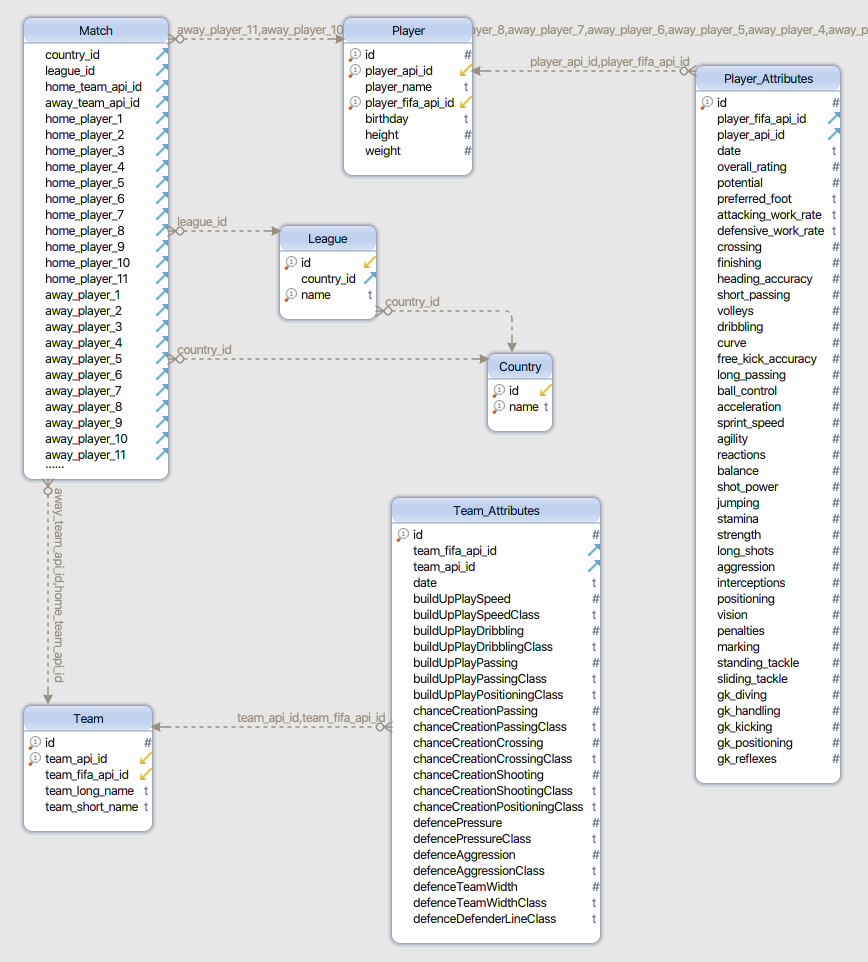
\includegraphics[scale=.5]{erm} % png ist Default für Dateiendung
\end{center}
\caption{Entity Relationship Modell European Soccer Database
%  \parencite[eigene Darstellung mit Übersezung in Anlehnung an][]{Hevner2007}
}
\end{figure}



%\chapter{Forschungsmethoden}
\label{cha:Forschungsmethoden}
%
In diesem Kapitel werden diejenigen Forschungsmethoden genannt, die in einer Abschlussarbeit an
\glspl{haw} am häufigsten anzuwenden sind. Dabei ist das \emph{Literaturreview} nach Abschnitt
\ref{sec:FM-Literaturreview} zwingend erforderlich. Oft sind dann entweder \emph{Evaluationen} gefordert,
für die sich die Ansätze aus Abschnitt \ref{sec:FM-Evaluationen} eignen. Zumeinst aber ist eine
(prototypische) Umsetzung gefordert, für die sich der \emph{Design Science Research} Ansatz nach
Abschnitt \ref{sec:FM-Design_Science} als Herangehensweise etabliert hat. Sowohl bei Evaluationen
als auch bei der prototypischen Umsetzung sind häufig \emph{Interviews} zu führen, wofür sich die
in Abschnitt \ref{sec:FM-Interviews} kurz beschriebene strukturierte Vorgehensweise anbietet.
%
\section{Literaturreview}
\label{sec:FM-Literaturreview}
%
Die Durchführung des Literaturreviews soll den Vorschlägen von \textcite{Webster2002} folgen.
Dabei sind die Ausführungen bis auf Verallgemeinerungen fast wörtlich einer Vorversion der Bachelorarbeit von 
\textcite{Riedel2018} entnommen und zeigen damit exemplarisch, wie man strukturiert an
das Literaturreview herangehen kann.

Im Rahmen einer Literaturrecherche wurden die Webdatenbanken ACM Digital Library,
Ebscohost, IEEE Xplorer sowie die akademischen Suchmaschinen Google Scholar und
Semantic Scholar nach relevanten Publikationen und Quellen durchsucht. Hierbei wurde
darauf geachtet Peer-Reviewed Journals und Peer-Reviewed Konferenzbeiträge als
Suchergebnisse zu erhalten, damit eine zuverlässige Forschung durchgeführt werden
konnte. Als Suchstring diente eine logische Kombination aus den Begriffen: „Begriff 1“ 
AND „Begriff 2“ OR „Begriff 3“ AND „Begriff 4“. Manche
Quellen wurden außerdem durch weitere Keywords identifiziert. Zusätzlich wurde nach
einem Publikationsdatumsintervall von „Startjahr -- Endjahr“ gefiltert, was die Suchresultate
näher spezifizierte. Ein Teil der Literaturrecherche war die Vorwärts- und
Rückwärtssuche, bei der auf Zitationsbasis weitere relevante Quellen entdeckt wurden.
Der Datumsfilter hatte hierauf einen positiven Effekt. Durch die Rückwärtssuche konnte
weitere Literatur identifiziert werden, die meist nicht viel älter als die Publikation, die
sie zitierte, war. Bei der Vorwärtssuche wurde hingegen Google Scholar verwendet.
Insgesamt haben sich auf diese Weise über $x$ Publikationen ergeben. Anhand Titel,
Abstract, Einleitung und Schluss wurden $y$ aussortiert wegen mangelnder Relevanz. $z$
Quellen davon, $z_1$ Journal Artikel, $z_2$ Konferenzbeiträge, $z_3$ Bücher, $z_4$ Manuals, 
$z_5$ Webquellen sowie $z_6$ generische Dokumente bilden somit das Grundgerüst dieser Arbeit.
Die entdeckten Quellen wurden stringent, wie von \citeauthor{Webster2002}
empfohlen, in einer Tabelle nach Inhalt und Relevanz sortiert. Hierzu wurde die erste
Forschungsfrage aus dem Forschungsdesign in folgende 4 Themenblöcke
aufgeteilt: 
%
\begin{compactitem}
\item Begriff 1,
\item Begriff 2,
\item Begriff 3 und
\item Begriff 4.
\end{compactitem}
%
Die Quellen wurden dann entsprechend den einzelnen Themenblöcken
zugewiesen. Zusätzlich dienten weitere Themenblöcke als Anhaltspunkte, welche jedoch
keinen Einfluss auf die Relevanz der Quellen ausübten. Zu jeder Quelle wurden die
Kernaussagen sowie inhaltsrelevante Punkte notiert. Die Quellen wurden nach der
Relevanz auf einer Skala 1 -- 4 bewertet, wobei 4 eine hohe Relevanz zu allen
Themenblöcken repräsentiert und 1 für eine geringe Relevanz steht. Daraus bilden sich
folgende Bewertungskriterien nebst Punktzahl:
\begin{itemize}
\item Alle vier Themenfelder sind umfassend behandelt oder beschrieben (4 Punkte)
\item Mindestens zwei Themenfelder sind umfassend abgedeckt und der Inhalt besitzt
  einen hohen Bezug zum Forschungsthema (3 Punkte)
\item Mindestens ein Themenfeld ist umfassend beschrieben und hat Bezug zum
  Forschungsthema (2 Punkte)
\item Behandelt ein Themenfeld oder trägt zum Forschungsthema bei (1 Punkt)
\end{itemize}

Es wurde außerdem die Anzahl der Zitate einer Publikation notiert, wodurch sich die
Signifikanz einer Quelle in der wissenschaftlichen Community bemessen lässt. Der
Verband der Hochschullehrer für Betriebswirtschaft e.\,V.~(VHB) bietet mit einem eigenen 
Ratingsystem (Jourqual)
eine gerankte Übersicht vieler Journals und Konferenzen an \parencite[s.][]{VHB2015}, wobei die
Skala von A+ (beste) bis D (mittelmäßig) reicht. Falls ein Journal oder eine Konferenz
kein Rating hatte, wurde stattdessen der Scimago Journal \& Country Rank (SJR), falls
vorhanden, genommen \parencite[s.][]{Scimago2004}. Diese Angaben unterstützten den oben
beschriebenen Bewertungsprozess.
Auf diese Weise resultierte ein tabellarisches Literaturreview, welches im Anhang 
\ref{anh:Anh-Literaturreview} sortiert 
nach Publikationstyp und Relevanz zu finden ist.

Nach diesen Ausführungen zu der elementaren Phase des Literaturreviews geht der folgende Abschnitt auf
Methoden für die Durchführung von Evaluationen ein -- einer häufigen Aufgabenstellung in Abschlussarbeiten.

\section{Evaluationen}
\label{sec:FM-Evaluationen}
%
Die Ausführungen dieses Abschnitts sind der Bachelorarbeit von \textcite{Oezen2018} entnommen und
lediglich leicht modifiziert (verallgemeinert) wiedergegeben.
%

Es gibt viele unterschiedliche Definitionen für die Evaluierung. Die \gls{degeval},
die sich um die Professionalisierung jeglicher Form von Evaluierung
bemüht, sieht die Evaluierung als eine strukturierte Vorgehensweise, um den Nutzen oder den
Wert eines Evaluationsgegenstandes zu untersuchen \parencite[s.][]{degeval2008}. Evaluationsgegenstände 
können demnach materieller, sowie nicht-materieller Natur sein, wie z.B. Software. Dabei müssen empirisch
gesammelte qualitative und/oder quantitative Daten die Basis für die erzielten Ergebnisse und Empfehlungen 
sein. 

Es gibt zwei Arten von Evaluierung: formative Evaluierung und summative Evaluierung. Die formative 
Evaluierung findet
während der Entwicklung des Evaluationsgegenstandes statt und beabsichtigt dessen Wert zu
verbessern oder dessen Effektivität zu steigern. Die summative Evaluierung ermöglicht den
Evaluatoren und Evaluatorinnen Erkenntnisse aus abgeschlossenen Aktionen zu erlangen. Die
meisten Evaluierungen ähneln sich laut \textcite{Hegner2003} in drei Punkten:
\begin{itemize}
\item Ausgangspunkt der Evaluierung ist der Evaluationsgegenstand, der untersucht werden
soll.
\item Der Evaluationsgegenstand soll Eigenschaften, die vor der Evaluierung formuliert
wurden, aufweisen.
\item Im Evaluationsprozess werden die formulierten Eigenschaften mit den tatsächlichen
Eigenschaften verglichen.
\end{itemize}

\subparagraph{\textrm{Evaluierungstechniken}}\footnote{%
Dies ist fett geschrieben, um mit einem Label später hier her springen zu können!}
%
\label{citedemo}
 helfen den Evaluatorinnen und Evaluatoren, die betrachteten
Evaluierungsgegenstände basierend auf den Ergebnissen einer quantitativen Analyse in eine
Rangfolge zu bringen \parencite[s.][]{Lai1999}. Nach \textcite{Jadhav2011} sind die beiden wohl 
am häufigsten benutzten Evaluierungstechniken der Analytische Hierarchieprozess und die
Nutzwertanalyse. Diese beiden Techniken gehören zu den klassischen Ansätzen der 
\gls{mcda} \parencite[s.][]{Geldermann2014}.

In den meisten Entscheidungsproblemen werden laut \citeauthor{Geldermann2014}
mehrere Ziele parallel verfolgt, die teilweise
konfliktär sein können oder abhängig voneinander sind.
Die MCDA-Methoden ermöglichen Entscheidungsträgern ein bestimmtes Ziel, also einen definierten
und angestrebten Zustand in der Zukunft, unter Berücksichtigung solcher konkurrierender
Alternativen zu erreichen \parencite[s.][]{Lai1999}.
Hinsichtlich der Auswahl von Software wird \zB meist das Ziel verfolgt, eine
einfach zu bedienende Software auszuwählen. Andererseits besteht oft ein Zielkonflikt darin, dass
die Software Funktionalitäten bieten soll, die gewisse komplexe Operationen ermöglichen. Die
gleichzeitige Betrachtung mehrerer Eigenschaften, um daraus eine Rangfolge der
vorhandenen Alternativen zu erstellen und die Beste aus ihnen zu wählen, machen den
Prozess der Evaluierung und Auswahl von Software zu einem multikriteriellen
Entscheidungsproblem \parencite[s.][]{Jadhav2011}. Dieser Prozess ist nach \textcite{Stamelos2000}
jedoch keine technische Aktivität, sondern eine subjektive und ungewisse Entscheidungsfindung.
Deshalb sollte dieser Prozess nicht als Automatisierung
der Entscheidungsfindung wahrgenommen werden. MCDA-Methoden nehmen den
Verantwortlichen nicht die Entscheidung selbst ab, sondern
helfen den Entscheidungsträgern ihr Verständnis für das Entscheidungsproblem zu
verbessern, indem sie das Problem strukturieren \parencite[s.][]{Geldermann2014}. 
Die Rangfolge gibt nur eine gute Vorstellung davon, welche Alternativen die besseren sind
\parencite[s.][]{Jadhav2011}. 
%
\subsection{Analytischer Hierarchieprozess}
\label{subsec:FM-Eval-Analytischer_Hierarchieprozess}
Der Analytische Hierarchieprozess (engl. Analytic Hierarchy Process) ist eine vom
Mathematiker \textsc{Thomas L. Saaty} eingeführte Methode, um komplexe multikriterielle
Entscheidungsprobleme zu unterstützen \parencite[s.][]{Saaty1990}. Die Methode ist flexibel und
mächtig und eignet sich sowohl für das Lösen von qualitativen als auch von quantitativen
multikriteriellen Entscheidungsproblemen. Sie unterstützt die individuelle Entscheidungsfindung
und ebenso Entscheidungen in einer Gruppe \parencite[s.][]{Lai2002}. Der
Analytische Hierarchieprozess ist vielfältig einsetzbar und findet Anwendung in weiten
Bereichen wie \zB beim Autokauf \parencite[s.][]{Byun2001}, bei der Händlerwahl 
\parencite[s.][]{Tam2001} und auch bei der Softwareauswahl \parencite[s.][]{Lai1999}.
%
\subsection{Nutzwertanalyse}
\label{subsec:FM-Eval-Nutzwertanalyse}
Die Nutzwertanalyse (engl. Weighted Scoring Method) ist eine Analysetechnik in der
Entscheidungstheorie und dient als Unterstützung bei der multikriteriellen Entscheidungsfindung \parencite[s.][]{Putzhammer2015}. Die Methode beinhaltet die Identifizierung von allen
projektrelevanten, nicht-monetären Kriterien, sowie die Verteilung der Gewichtungen für
jedes Kriterium und die Vergabe von Punkten für jede Option \parencite[s.][]{Windolph2015}. Die
Gewichtungen spiegeln die relative Wichtigkeit der Kriterien gegeneinander wider. Die Punkte
dagegen repräsentieren das Abschneiden der Optionen in Bezug zu den Kriterien. Das Ergebnis
ist ein gewichteter Nutzen für jede einzelne Option.
%
\subsection{Ergebnisdarstellung}
\label{subsec:FM-Eval-Ergebnisdarstellung}
%
Um die Ergebnisse einer Evaluation übersichtlich und kompakt darzustellen, eignen sich insbesondere
\emph{(Spinnen-)Netzdiagramme}. Alternativ können auch \emph{gestapelte Säulendiagramme} eingesetzt
werden.

Während die in diesem Abschnitt behandelten Evaluationen recht häufig in Abschlussarbeiten durchzuführen
sind, gilt dies im Umfeld von Informationssystemen an \glspl{haw} noch mehr für die prototypische
Umsetzung eines IT-Artefakts. Daher widmet sich der folgende Abschnitt einer hierfür geeigneten
Forschungsmethode.
%
\section{Design Science}
\label{sec:FM-Design_Science}
%
Dieser Abschnitt folgt erneut einer Vorversion der Bachelorarbeit von \textcite{Riedel2018} und
wird für die Zwecke dieser Vorlage wiederum aqäquat modifiziert.
%

Oftmals ist dies die zentrale Forschungsmethode, nämlich immer dann, wenn ein \emph{Proof of Concept} oder ein \emph{Prototyp} erstellt werden soll. Daher kommt der \Fachbegriff{Design Science Research} Ansatz von
\textcite{Hevneretal2004}
als zentrale Forschungsmethode zum Einsatz. Mit dem \Fachbegriff{Information System Research Framework}
wird laut diesen Autoren eine Art Best Practice für praxisorientierte Problemstellungen geschaffen. 
Als zentraler Baustein gilt hierbei das IT-Artefakt, wobei
IT-Artefakte Methoden, Modelle oder Prototypen sein können. Weiterhin wird das
Framework in Behavioral Science und Design Science unterteilt. Bei der Behavioral
Science steht die Theorieentwicklung und –validierung im Vordergrund, während bei der
Design Science das konkrete IT-Artefakt die betrieblichen Anforderungen erfüllen soll. 
Meistens sind beide Paradigmen für Design Science Research Projekte erforderlich, wobei
bei einer prototypischen Implementierung der reine Design Science Ansatz und das IT-Artefakt 
im Fokus stehen.

\textcite{Iivari2007} kritisiert in einem Forschungsbeitrag die oben beschriebenen Paradigmen.
Hierzu entwarf der Autor 12 Thesen. Unter diesen 12 Thesen befindet sich beispielsweise
eine, die besagt, dass der Wertbeitrag des Design Science Forschungsprojekts eindeutig
erkennbar sein sollte. Ein weiterer Kritikpunkt an der Arbeit von \textcite{Hevneretal2004} war die
unzureichende Beschreibung, wie ein IT-Artefakt explizit entwickelt werden soll. 
\textcite{Hevner2007} nahm sich dieser Kritik an 
und entwickelte ein neues Framework, das die 12 Thesen von \textsc{Iivari} berücksichtigt.
% Abbildung \ref{fig:ThreeCycleView} -> eigener Befehl
\abbildung{ThreeCycleView} zeigt dieses Framework. Hinzugekommen sind 3 iterative Prozesse,
die Zyklen genannt werden. Diese drei Zyklen werden nachfolgend in Anlehnung an \textcite{Hevner2007}
kurz beschrieben.
%
\begin{figure}[H]
\label{fig:ThreeCycleView}
\begin{center}
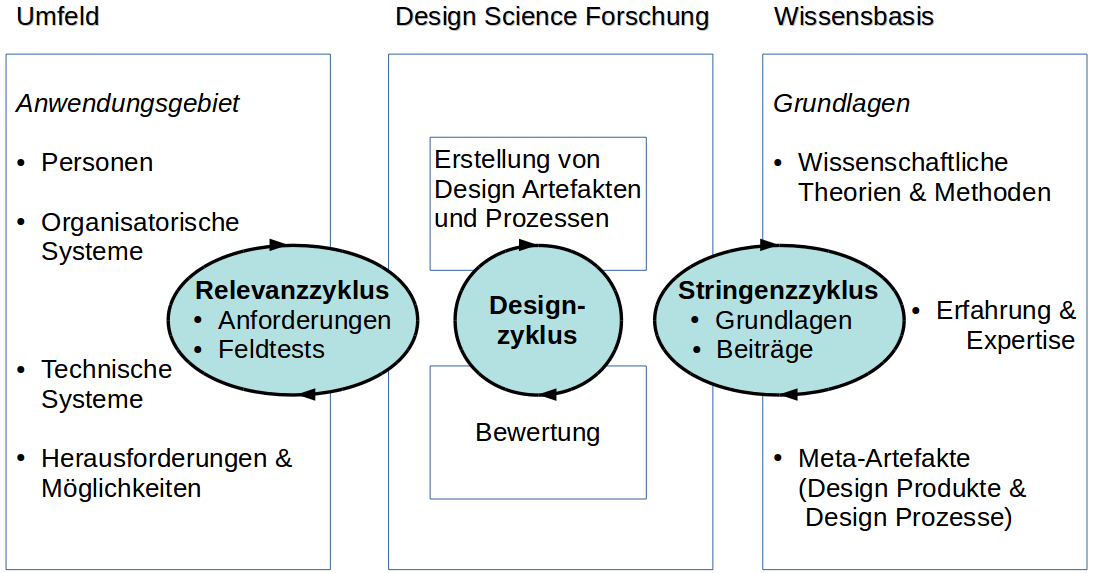
\includegraphics[scale=.3]{Drei_Zyklen_Sicht} % png ist Default für Dateiendung
\end{center}
\caption{Die drei Zyklen der Design Science Research
  \parencite[eigene Darstellung mit Übersezung in Anlehnung an][]{Hevner2007}}
\end{figure}
%
Der \Fachbegriff{Relevanzzyklus} (engl.~\Fachbegriff{Relevance Cycle}) bildet den Anfang eines 
Design Science Forschungsprojektes. In
diesem ersten iterativen Vorgang sollen die Anforderungen sowie der
Anwendungsbereich ermittelt werden. Insbesondere gilt es hier die Akzeptanzkriterien
für das vom Forscher zu erstellende IT-Artefakt zu definieren. Das fertige IT-Artefakt
kann dann wieder in das Umfeld eingebracht werden, wo es
anhand der definierten Kriterien evaluiert und getestet wird. Je nach Testergebnis und Feedback der
Stakeholder können neue Anforderungen entstehen und zusätzliche Iterationen
notwendig sein.

Der \Fachbegriff{Designzyklus} (engl.~\Fachbegriff{Design Cycle}) bildet den zentralen Zyklus 
der \Fachbegriff{Drei-Zyklen-Sicht} (engl.~\Fachbegriff{Three-Cycle-View}; s. \abbildung{ThreeCycleView}).
Dieser Zyklus wird am häufigsten iteriert, da er die Brücke zwischen dem Umfeld, in dem
das Artefakt eingesetzt wird (Relevanzzyklus), und der Wissensbasis
(Stringenzzyklus) bildet. Die Anforderungen für das IT-Artefakt kommen aus dem
Relevanzzyklus und die Methoden zur Erstellung und Evaluierung des Artefakts aus dem
Stringenzzyklus.

Der \Fachbegriff{Stringenzzyklus} (engl.~\Fachbegriff{Rigor Cycle}) greift auf eine Wissensbasis
zu, die dem Forscher
verschiedene Methoden und Werkzeuge anbietet. Dadurch soll das Projekt
einen wissenschaftlichen Stellenwert erreichen. Der Forscher erstellt mit diesem
Methodenfundus sein IT-Artefakt im Designzyklus. Dabei soll das IT-Artefakt einen
wissenschaftlichen Beitrag zur Wissensbasis leisten, indem es dem akademischen
Publikum zugänglich wird.

Jedes Forschungsprojekt, welches gemäß dem Design Science Forschungsansatz durchgeführt wird,
bedarf einer angepassten Ausprägung desselben. Hierzu können die in \tabelle{DSResearchGuidelines}
aufgelisteten Richtlinien nach \textcite{Hevneretal2004} dienen.
%
{\small
\begin{longtable}{p{.26\textwidth}p{.33\textwidth}p{.32\textwidth}}
\toprule
\textbf{Richtlinie} & \textbf{Kurzbeschreibung} & \textbf{Erzielt durch} \\
\midrule
1: Artefakt-Design & Design Science Research muss ein realisierbares Artefakt herstellen &
Prototypische Implementierung  \\*
\midrule
2: Problemrelevanz & Technologische Lösung zu einem relevanten, betrieblichen Problem &
problemspezifische Methode \\*
\midrule
3: Designbewertung & Mehrwert des Artefakts muss umfassend getestet werden & 
problemangepasster Validierungscheck  \\*
\midrule
4: Forschungsbeitrag & Verifizierbare, eindeutige Beiträge zur Forschung müssen erzielt werden &
konkreter Prototyp \\*
\midrule
5: Stringenz der\newline\phantom{5:} Forschung & Eindeutig nachvollziehbare Methoden zur
Erstellung und Evaluation des Artefakts & angewendete Forschungsmethoden  \\*
\midrule
6: Design als \newline\phantom{6:} Rechercheprozess & Suche nach einem effektiven Artefakt
erfordert Feedback und Methoden & Rücksprache mit Stakeholdern \\*
\midrule
7: Forschungs-\newline\phantom{7:} vermittlung & Design Science Research muss den Zielgruppen verständlich präsentiert werden &
strukturierte und nachvollziehbare Dokumentation \\*
\bottomrule \\
\caption{Die sieben Design Science Forschungsrichtlinien gemäß \textcite{Hevneretal2004}}
\label{tab:DSResearchGuidelines}
\end{longtable}
} % end \small
%
Dabei ist festzuhalten, dass diese Richtlinien keine feste Sequenz bilden, sondern als
voneinander unabhängig und sich ergänzend betrachtet werden können. Sie sind geeignet, den
Design Science Research Prozess zu unterstützen.

Ergänzend können bei Evaluationen oder im Relevance Cycle des Design Science Resaerch Prozesses
auch Experteninterviews eine Rolle spielen. Einer strukturierten Herangehensweise an diese widmet
sich der folgende Abschnitt.
%
\section{Interviews}
\label{sec:FM-Interviews}
%
Bei manchen Aufgaben sind strukturierte Interviews gefragt. Auch dieser Abschnitt folgt wiederum 
mit Anpassungen einer Vorversion der Bachelorarbeit von \textcite{Riedel2018}.
%

Mit dem Experteninterview als weitere Forschungsmethode können wichtige Inhalte wie
Anforderungen einer Anwendung, Zielsetzungen eines Projekts oder Probleme eines
Prozesses in einem zu untersuchenden Unternehmen festgestellt werden. Im Unterschied
zur quantitativen Umfrage erfolgt das Experteninterview qualitativ, d.h. die Aussagen
eines einzelnen interviewten Experten gelten als anerkannt und empirisch belegt
%
% mehrere Zitate in einem Befehl
%
\parencites[s.][103]{Glaeser2010}{Mayring1994}.
%
Eine genaue Definition, ab wann ein Experte als
Experte gilt, wird in der Literatur kontrovers diskutiert. Nach \textcite{Mieg2006} ist
ein Experte eine Person im Unternehmen, die mindestens 10 Jahre Erfahrung auf dem
untersuchten Gebiet hat. An anderer Stelle wird betont, dass ein Experte vor allem eine
hohe Expertise zu den befragten Themen haben sollte und die reine Erfahrungszeit nicht
maßgebend sei \parencite[s.][11 -- 12]{Glaeser2010}. Es kann daher durchaus begründet werden, 
Interviews mit Experten zu führen, die zwar nicht alle die 10 Jahres Grenze erreicht haben,
aber dennoch ein fundiertes Wissen über den Anwendungsfall besitzen.

Zur Durchführung des Interviews ist ein durchdachter Leitfaden notwendig an dem sich
das Gespräch orientiert \parencite[s.][142 -- 143]{Glaeser2010}. Dabei existieren
unterschiedliche Varianten eines Interviewleitfadens. Neben der Möglichkeit, falls vorhanden,
ein standardisiertes Leitfadeninterview zu verwenden, kann auch ein eigener Leitfaden
entwickelt werden, bei dem ein Teil der Fragen deduktiv aus der Theorie
heraus gebildet wird und ein anderer Teil der Fragen sich im Verlauf des Interviews ergibt
\parencite[s.][42]{Glaeser2010}. Eine Leitfrage soll hierbei nach \textsc{Gläser} und \textsc{Laudel}
das Wissen für ein konkretes Thema, Problem oder Forschungsfrage beschaffen. Aus
diesen Überlegungen heraus lässt sich dann ein Framework für Interviewleitfäden wie in
Tabelle \ref{tab:Interviewleitfaeden} dargestellt ableiten.

%
\begin{table}[h]
\label{tab:Interviewleitfaeden}
\begin{tabular}{llllc}
\toprule
\textbf{Leitfrage} & \textbf{Teilfrage} & \textbf{Zweck} & \textbf{Notizen} & \textbf{Ok} \\
\midrule
1. Erste Leitfrage & \parbox[c][10ex]{0pt}{} 1.1 Teilfrage & -- erwartete Antwort & & \\
\cmidrule{2-3}
                 & \parbox[c][10ex]{0pt}{} 1.2 \emph{Schlüsselfrage} & -- Ziel der Frage & (optional) & \Square                 \\ \cmidrule{2-3}
& \parbox[c][10ex]{0pt}{} 1.3 Teilfrage & \ldots & & \\
\midrule
2. Zweite Leitfrage & \parbox[c][10ex]{0pt}{} 2.1 Teilfrage & \ldots & (optional) & \Square \\
\bottomrule\\
\end{tabular}
\caption{Framework für Interviewleitfäden}
\end{table}
%
Es zeigt eine Unterteilung der Leitfragen in
Teilfragen, die die
übergeordnete Frage umfassend beantwortet. Schlüsselteilfragen sind hierbei Fragen, die
vom Interviewten in jedem Fall zu beantworten sind. Jede vordefinierte Teilfrage erzielt
einen bestimmten Output, der ebenfalls notiert werden sollte. Eine Spalte für Notizen
ermöglicht bereits während des Interviews wichtige Informationen zu notieren. Das
Framework kann als Grundlage für die Interviewleitfäden einer Arbeit dienen.
Ein Experteninterview sollte während der Durchführung aufgezeichnet werden, damit
wichtige Inhalte später noch einmal angehört werden können und eine Aufbereitung des
Gesprächsinhalts ermöglicht wird \parencite[s.][42]{Glaeser2010}. 
Nach den Interviews erfolgt die qualitative Inhaltsanalyse nach
\textcite{Mayring2010}. 

Die Auswertungsmethode sieht dabei zwei mögliche Vorgehensweisen vor:
%
\begin{compactenum}
\item die explizierende Transkription bei der das komplette Gespräch transkribiert wird und
\item die zusammenfassende Inhaltsanalyse bei der nur die inhaltsrelevanten Aussagen transkribiert werden.
\end{compactenum}
%
Meist ist Letzteres praktikabel. Zur Auswertung werden außerdem einzelne zentrale
Aussagen zu deduktiv oder zu induktiv gebildeten Kategorien zugeordnet \parencite[s.][]{Mayring2010}.
Dadurch wird eine Übersicht über die zentralen Aspekte des Interviews ermöglicht. Abbildung 
\ref{fig:Interviewkategorien} zeigt den Unterschied beider Kategorienbildungen.
%
\begin{figure}[H]
\label{fig:Interviewkategorien}
\begin{center}
\includegraphics[scale=.4]{Kategorien_Mayring}
\end{center}
\caption{Kategorienbildung induktiv (links) und deduktiv (rechts) \parencite[eigene Darstellung nach][]{Mayring1994}}
\end{figure}
%
Aus Abbildung \ref{fig:Interviewkategorien} lässt sich ableiten, dass die Kategorien bei der
induktiven Bildung anhand des Ausgangsmaterials, dem Interview, gebildet werden und bei der
deduktiven Variante die Bildung der Kategorien durch vorausgegangene theoretische
Überlegungen erfolgt. Auf eine formale Reliabilitätsprüfung sowie auf einen Kodierleitfaden
wird der Einfachheit halber verzichtet.
Mit Experteninterviews und der zusammenfassenden Inhaltsanalyse werden die
Anforderungen der neuen Anwendungslösung im untersuchten Unternehmen empirisch
erhoben und somit eine prototypische Umsetzung (bei einem Design Science Forschungsprojekt)
oder eine Auswahl zwischen Alternativen (bei Evaluationen)
gemäß dieser Kriterien ermöglicht.
%
\section{Data Science Vorgehensmodelle}
\label{sec:FM-DataScienceVorgehen}
%
Für Abschlussarbeiten mit Bezug zu \emph{Data Science} empfiehlt sich die Strukturierung des
Hauptteils der Arbeit nach dem Literaturreview gemäß einem etablierten Vorgehensmodell für
Data Science Aufgaben. Hier wird zumeist auch heutzutage noch der \gls{crispdm} verwendet,
auch wenn dieser in seiner ursprünglichen Form nicht mehr ganz auf der Höhe der Zeit ist. Es
gibt den zugehörigen Guide auch seit längerem nur noch über das \emph{Internet Archive} zu
beziehen \parencite[s.~][]{Chapman1999}.

Mittlerweile gibt es verschiedene Weiterentwicklungen von CRISP-DM, die versuchen, sowohl technischen
Neuerungen wie Cloud Computing oder Big Data aber auch modernen Ansätzen wie agilem
Projektmanagement Rechnung zu tragen. Dazu gehört auch der \Fachbegriff{Team Data Science Prozess}
von \textcite{Microsoft2018}. Die Phasen 2 -- 4 dieses Prozesses, also \emph{Datenerfassung und -auswertung},
\emph{Modellierung} und \emph{Bereitstellung} eignen sich zumeist auch gut für die Strukturierung des
Hauptteils einer Abschlussarbeit mit einer Aufgabenstellung aus dem Bereich Data Science. Daher
ist dieser Prozess als Leitlinie sowohl für die Umsetzung als auch für das Schreiben der Abschlussarbeit
bei derartigen Projekten gut geeignet.

Nach der Darstellung etablierter Forschungsmethoden für praktische Aufgabenstellungen in
Abschlussarbeiten geht es im folgenden Kapitel um 
%
\todo[color=red!40, size=\tiny]{Überleitung fertig formulieren!}
%ein weiteres essenziell wichtiges Thema bei
%der Erstellung von Abschlussarbeiten, nämlich um das Zitieren.
%\chapter{Zitate und Referenzen}
\label{cha:ZitateReferenzen}
% 
Dieses Kapitel beschäftigt sich mit Verweisen -- zum einen mit internen, aber zum anderen und im Besonderen
mit dem Verweis auf verwendete Quellen durch Zitieren. Eine \gls{faq} in diesem Zusammenhang ist die nach 
dem \Fachbegriff{Zitationsstil}. 
%
\todo{Welche Zitationsstile sind möglich?} 
%

Daneben geht es auch um besondere Formen interner Referenzen, etwa für besondere Verzeichnisse. Ferner
gibt es einige weitere Hinweise, etwa zum \gls{doi} oder auf Software zur Verwaltung der Quellen.

Außerdem werden in der
Quelldatei \Datei{Inhalt/ZitateReferenzen.tex} auch einige der in der Datei \Datei{Formales/Befehle.tex} 
definierten eigenen Befehle verwendet, um auch dies zu exemplifizieren.
%
\section{Zitate}
\label{sec:ZR-Zitate}
%
Zunächst einmal sind beim Zitieren bestimmte \emph{Prinzipien} zu beachten. Das sicher wichtigste
dieser Prinzipien lautet:
%
\begin{quote}
\textsl{Hat man etwas aus Quellen
übernommen (Text, Ideen, Abbildungen, Code, etc.), so muss man die Quelle auch angeben!}
\end{quote}
%
Anderenfalls handelt es sich um ein \gls{plagiat}, was insbesondere bei Vorsatz zur Bewertung der
Abschlussarbeit mit \textbf{ungenügend} führt!

Hinsichtlich Zitaten stellt sich außerdem immer die Frage nach dem \emph{Stil}. Oftmals wird mit Fußnoten
gearbeitet, was aber nicht den Vorgaben entspricht. Eigentlich handelt es sich lediglich um eine einzige:
%
\begin{quote}
\textsl{Es ist der \Fachbegriff{Harvard-Stil}, auch \Fachbegriff{Autor-Jahr-Zitierweise} genannt, mit
Kurzbelegen zu verwenden! \parencite[s.][]{Wikipedia2010}}
\end{quote}
%
Wie dies umzusetzen ist, kann man bereits in den Kapiteln \ref{cha:Einleitung} und \ref{cha:Forschungsmethoden}
in Verbindung mit dem Literaturverzeichnis sehen. Dort erkennt man eine weitere Anforderung, nämlich:
%
\begin{quote}
\textsl{Reine Onlinequellen sind von wissenschaftlichen Quellen wie Büchern und Artikeln in 
(wissenschaftlichen) Publikationen zu trennen!}
\end{quote}
%

Weitere nützliche Hinweise zum korrekten Zitieren findet man auf der Website der Uni Ulm 
bei \textcite{Hoelting2018}. Zusätzlich ist auch zu beachten, dass man keine \Fachbegriff{Blindquellen}
ins Literaturverzeichnis aufnimmt, \dh keine Quellen, die nicht auch wirklich in der Arbeit zitiert
werden. Um dies sicher zu stellen ist eine weitere Anforderung:
%
\begin{quote}
\textsl{Im Literaturverzeichnis sind Rückverweise zu verwenden!}
\end{quote}
% 
Dies bedeutet, dass im Literaturverzeichnis bei den Quellen anzugeben ist, auf welcher Seite der Arbeit
sie verwendet wurden. Mehr zum Thema Rückverweise findet sich in Abschnitt \ref{subsec:ZR-BR-Rueckverweise}.
%
\todo{Das obige ToDo kann weg} 
%
\section{Besondere Referenzen}
\label{sec:ZR-BesondereReferenzen}
%
Es werden bei Verwendung dieser \LaTeX{}-Vorlage auch Referenzen für das Abkürzungs- und Symbolverzeichnis
sowie für das Glossar erzeugt (Informationen hierzu findet man in kompakter Form bei \textcite{Partosch2015}).
Ferner wird aus dem Literaturverzeichnis heraus auf die Seiten zurückverwiesen, auf denen ein Zitat vorkommt.
Diese Arten von besonderen Referenzen sollen hier kurz diskutiert werden.

Dabei werden Abkürzungen, Symbole und Glossar mit Hilfe des Pakets \Paket{glossaries} und den zugehörigen
Befehlen wie etwa \Code{\bs{}gls\{\}} erzeugt, während für
die Rückverweise eine Kombination von Optionen in den Paketen \Paket{biblatex} und \Paket{hyperref} 
verantwortlich sind.
%
\subsection{Abkürzungen}
\label{subsec:ZR-BR-Abkuerzungen}
%
Auch für Abkürzungen ist eine wichtige Regel zu beachten:
%
\begin{quote}
\textsl{Bei der ersten Verwendung einer Abkürzung / eines Akronyms im Text ist
der Begriff zusätzlich auszuschreiben bzw.~zu erklären!}
\end{quote}
%
Abkürzungen werden bei dieser Vorlage, wie Symbole und Glossareinträge auch, in einer speziellen Datei,
nämlich \Datei{Inhalt/Glossar.tex}, gesammelt.
Ein Beispiel ist das Akronym \gls{degeval}. Man beachte, dass bei der ersten Verwendung weiter oben
automatisch der ausgeschriebene Begriff verwendet wurde, während später, wie \zB hier, lediglich
das Akronym kommt,
so wie vorgeschrieben. In jedem Fall wird im PDF auf das Abkürzungsverzeichnis referenziert. Ein
Abkürzungsverzeichnis wird erwartet!
%
\subsection{Symbole}
\label{subsec:ZR-BR-Symbole}
%
Die folgenden Symbole werden exemplarisch definiert und dann ins Symbolverzeichnis übernommen:
zunächst das \gls{kappa} und dann das \gls{datenbasis}. 
%
\subsection{Glossar}
\label{subsec:ZR-BR-Glossar}
%
Das Glossar ist ein besonderes Verzeichnis, in dem man wichtige Begriffe bei Bedarf näher erläutern kann. Wie
das Symbolverzeichnis ist es optional, während ein Abkürzungsverzeichnis eigentlich immer nötig ist. 
%
\subsection{Rückverweise}
\label{subsec:ZR-BR-Rueckverweise}
%
Eine interessante Option für das Literaturverzeichnis sind Rückverweise auf die Seite, auf der die Verweise
erfolgt sind. Dies wird, wie in Abschnitt \ref{sec:ZR-Zitate} erwähnt, auch explizit verlangt, um die
Angabe von Blindquellen auszuschließen.
Für die korrekte Umsetzung mit \LaTeX{} sind sowohl im Paket \Paket{biblatex} die Option \Code{backref} und im
Paket \Paket{hyperref} verschiedene Optionen zu setzen (siehe Datei \Datei{Formales/Packages.tex}).
Darüberhinaus muss man noch in der Hauptdatei \Datei{Abschlussarbeit.tex} mit dem
\Code{\bs{}pagenumbering}-Befehl geschickt arbeiten (siehe dort). Tut man dies nicht, so werden zwar die
Seitenzahlen korrekt im Literaturverzeichnis angegeben, aber die Verweise im PDF sind inkorrekt.
%

Abschließend soll noch erwähnt werden, dass offensichtlich auch interne Verweise auf Abschnitte oder
bestimmte Positionen möglich sind. Dafür ist die Vergabe einer Markierung mittels \Code{\bs{}label\{name\}}
notwendig und die spätere Referenzierung mittels \Code{\bs{}ref\{name\}} oder \Code{\bs{}pageref\{name\}} 
(bzw.~\Code{\bs{}autoref\{name\}} in Verbindung mit dem \Paket{hyperref}-Paket). 
So kann man etwa den Unterschied beim Zitieren zwischen den Befehlen \Code{\bs{}textcite} und 
\Code{\bs{}parencite} im \autoref{citedemo} sehen.
%
\section{Weitere Hinweise}
\label{sec:ZR-WeitereHinweise}
%
%
\subsection{Trennung nach Quellenart}
\label{subsec:ZR-WH-Trennung}
%
Um die Anforderung nach Trennung von Online-Quellen und Büchern / (wissenschaftlichen) Publikationen umzusetzen
wird in dieser Vorlage einfach das Schlüsselwort \Code{internet} für Internetquellen verwendet und dieses dann
beim Erzeugen des Literaturverzeichnisses als Diskriminator nutzt. In der Hauptdatei
\Datei{Abschlussarbeit.tex} sieht das dann in den Zeilen 138 -- 144 wie in \listing{QuellenTrennung} aus:\\
%
\todo[size=\footnotesize]{Zei\-len\-num\-mern prüfen!!}
%
% Als Hintergrund eine Farbe mit Namen (dvipsnames), und davon nur 30%
%
\lstinputlisting[firstline=138, lastline=144, language={[LaTeX]TeX}, %
 caption={Trennung der Quellenarten}, backgroundcolor=\color{SkyBlue!30}, %
 emph={notkeyword,keyword}, emphstyle=\color{YellowOrange}, %
 label=lst:QuellenTrennung,
]{Abschlussarbeit.tex}
%
\paragraph{Umgang mit URLs} 
\label{para:urls}%
Diese sollten bei Büchern und Publikationen \emph{nicht} mit angegeben werden, während
sie bei Online-Quellen natürlich essenziell sind. Daher kann man hier nicht allgemein die Option setzen, um URLs
komplett aus dem Literaturverzeichnis zu verbannen. Allerdings sollte die URL-Information auch nicht ganz unter
den Tisch fallen, zumindest in der Literaturdatei sollte sie vorhanden sein. Daher ist diese in Quellen, die keine
Online-Quellen sind, im \emph{Kommentarfeld} zu hinterlegen.

Gleiches gilt für den Fall, dass eine URL einer Internetquelle im Literaturverzeichnis als deutlich zu lang
empfunden wird oder gar von \LaTeX{} nicht richtig umgebrochen werden kann. In diesem Fall benötigt man allerdings
einen Ersatz in Form eines \Fachbegriff{Shortlinks}, den man beispielsweise mit \textsf{Bitly} 
(\url{https://bitly.com/}) oder \textsf{Google} (\url{https://goo.gl/}) erzeugen kann.
%
\subsection{Verwendung von DOI}
\label{subsec:ZR-WH-DOI}
%
Neuere Bücher und (wissenschaftliche) Publikationen verwenden \glslink{doi}{DOI} als eindeutigen Identifikator
der Quelle. Daher sollte dieser, falls vorhanden, auch in der \emph{Literatur\underline{datei}}, aber
\textbf{nicht} im \emph{Literaturverzeichnis} auftauchen.

Es ist jedoch \emph{Vorsicht geboten}, denn diese DOI stimmen nicht immer (gerade bei älteren Publikationen) und sollten somit auf jeden Fall überprüft werden, denn fehlerhafte DOI in der Literaturdatei führen zur
Abwertung.
%
\subsection{Software}
\label{subsec:ZR-WH-Software}
%
Neben einer \gls{ide} für das Erstellen der \LaTeX{}-Dateien (wie etwa \Software{TeXmaker} (siehe Abschnitt
\ref{subsec:texmaker}) ist auch eine Software für die Verwaltung Ihrer Quellen zu verwenden. Hierbei 
ist eine klare Empfehlung \Software{JabRef}, ein plattformunabhängiges Java-Programm mit umfangreicher
Funktionalität (siehe Abschnitt \ref{subsec:jabref}).

Man beachte, dass \Software{JabRef} die Möglichkeit bietet, direkt aus dem Programm heraus eine
beträchtliche Anzahl an Internetportalen für wissenschaftliche Publikationen zu recherchieren
und anschließend die gefundenen Quellen
direkt zu übernehmen (sowie diese an die \LaTeX{}-\gls{ide} zu \emph{pushen}).

Eine kompakte Einführung mit Beispielen für Internetrecherche und Betrachtung verschiedener 
Literaturverwaltungssoftware gibt \textcite{Partosch2011}. Hier wird allerdings noch Bib\TeX{} verwendet.
Den Umgang mit \Paket{biblatex} mit \Paket{biber}-Backend behandelt \textcite{Pospiech2011} oder
(neuer) \textcite{Frank2017}. Dort findet man auch noch viele weitere Kursteile mit Übungen.
%

\underline{\emph{Bemerkung:}} Die beiden oben genannten Tutorials wurden ebenfalls mit \LaTeX{}
erstellt, nämlich mit dem Paket \Paket{latex-beamer}.
%

In jedem Fall gilt:
%
\begin{quote}
\textsl{Es ist ein Quellenverzeichnis im Bib(La)\TeX{}-Format in elektronischer Form mit abzugeben!}
\end{quote}
%

In den vorangegangenen beiden Kapiteln wurden allgemeingültige Informationen für Abschlussarbeiten
hinsichtlich der einzusetzenden
Forschungsmethoden sowie des Zitierens und anderer Arten von Verweisen gegeben, wobei in diesem Zusammenhang
natürlich bereits zahlreiche \LaTeX{}-Elemente exemplarisch verwendet wurden. Im nächsten Kapitel wird nun auf
spezielle Elemente nochmals näher eingegangen.
%
\todo[color=green!30]{übergeleitet!}
%

%\chapter{Umgang mit \LaTeX}
\label{cha:Umgang}
%
% Hier wird \input statt \include benötigt, da \include nicht geschachtelt werden darf ...
%
\section{Bilder, Tabellen und Listings}
\label{sec:BilderTabellenListings}
%
Für \LaTeX{} handelt es sich bei allen drei Arten von Objekten um sogenannte \Fachbegriff{Gleitobjekte}
(engl.~\emph{floats}), die beim Setzen an Stellen verschoben werden, wo sie am besten passen (im Falle
der Listings ist dies optional). 
Speziell bei Tabellen helfen die Pakete \Paket{booktabs} und \Paket{longtable}.
%
\subsection{Abbildungen}
\label{subsec:Abbildungen}
%
Bislang wurden in diesem Dokument zwei Abblidungen, nämlich \abbildung{ThreeCycleView} und 
\abbildung{Interviewkategorien}, verwendet. Hierbei wurden jeweils \emph{Screenshots} eingebunden. Allerdings
wurde dabei auch darauf geachtet, dass diese nicht einfach aus einem gefundenen PDF herauskopiert wurden, sondern
die Bilder wurden selbst erstellt. Das führt meist zu wesentlich besser lesbaren Abbildungen.

Besonders gut lesbar sind natürlich \Fachbegriff{Vektorgrafiken}. Diese lassen sich direkt in \LaTeX{} mit 
Hilfe des Pakets \Paket{tikz} erstellen, welches extrem mächtig ist. Viele Beispiele findet man hierzu auf
der Webseite \url{www.texample.net} und natürlich auch im zugehörigen (über tausendseitigen) Handbuch. 

\begin{figure}[H]
\begin{center}
\begin{tikzpicture}[scale=.45]
  \begin{scope}[blend group = soft light]
    \fill[red!30!white]   ( 90:1.2) circle (2);
    \fill[green!30!white] (210:1.2) circle (2);
    \fill[blue!30!white]  (330:1.2) circle (2);
  \end{scope}
  \node [font=\tiny] at ( 90:2)    {Typography};
  \node [font=\tiny] at ( 210:2)   {Design};
  \node [font=\tiny] at ( 330:2)   {Coding};
  \node [font=\footnotesize] {\LaTeX};
\end{tikzpicture}
\end{center}
\caption{Mit \Paket{tikz} erstellte Abbildung (eigene Darstellung)}
\label{fig:tikz}
\end{figure}
%
Dieses muss man natürlich nicht vollständig lesen, um mit \Paket{tikz} ansprechende Grafiken wie in 
\abbildung{tikz} erstellen zu können (das Original findet man bei \url{http://www.texample.net/tikz/examples/venn/}
und die obige \glqq Quellenangabe\grqq{} ist damit geflunkert \frownie).

%
Vielleicht sollte man noch weitere Abbildungen einfügen? Dann kann man sich auch eine Erinnerung setzen, damit das in der ToDo-Liste auftaucht.
%
\missingfigure{Da muss noch eine Abbildung hin}
%
Dies ist oft hilfreich, wie andere ToDos auch.
%
\subsection{Listings}
\label{subsec:Listings}
%
In Abschnitt \ref{subsec:ZR-WH-Trennung} hatten wir bereits ein Listing gesehen, welches aus einer
Datei eingelesen wurde. Das muss aber nicht sein, wie man am folgenden Beispiel sieht, welches der
Masterarbeit von \textcite{Walcher2014} entnommen wurde und direkt in der \LaTeX{}-Datei reproduziert
wird.

%
% Listing direkt hier eingefügt
\lstset{basicstyle=\footnotesize, showstringspaces=false}
\begin{lstlisting}[label=lst:bs4,caption=Einlesen einer Webseite mit \Paket{BeautifulSoup}]
from bs4 import BeautifulSoup
import urllib2
seite = urllib2.urlopen("http://blog.metropolsolar.de/")
seiteHtml = seite.read()
seite.close()
soup = BeautifulSoup(seiteHtml)
\end{lstlisting}

Besonders interessant ist die Möglichkeit, Listings mit \Paket{tikz}-Bildern zu kombinieren wie im Beispiel 
von \listing{tikzfiglst}
(leicht angepasst übernommen von \url{http://www.texample.net/tikz/examples/tikz-listings/}).
%
\newpage
\phantom{xyz}\vspace{1cm}
%
\begin{lstlisting}[language = C++, numbers = none, escapechar = !,
    basicstyle = \ttfamily\bfseries, xleftmargin=.2\linewidth, xrightmargin=.2\linewidth,
    frame=tb, tabsize=1, framesep = 3pt, framerule =.4pt,
    backgroundcolor = \color{white}, caption=Ein Listing kombiniert mit \Paket{tikz}-Bild, label=lst:tikzfiglst] 
 int!
   \tikz[remember picture] \node [] (a) {};
 !puissance!
   \tikz[remember picture] \node [] (b) {};
 !(int x,!
   \tikz[remember picture] \node [] (c){};
 !int n) { 

     int i, p = 1; !\tikz[remember picture] \node [] (d){};!           

     for (i = 1; i <= n; i++) 
       p = p * x; !\tikz[remember picture] \node [inner xsep = 40pt] (e){};! 

     return p; !
       \tikz[remember picture] \node [] (f){};!  
 }
\end{lstlisting}
\begin{tikzpicture}[remember picture, overlay,
    every edge/.append style = { ->, thick, >=stealth,
                                  Gray!60, dashed, line width = 1pt },
    every node/.append style = { align = center, minimum height = 10pt,
                                 font = \small\bfseries, fill= green!20},
                  text width = 2.9cm ]
  \node [above left = .75cm and -.75 cm of a,text width = 2.2cm]
                             (A) {return value type};
  \node [right = 0.25cm of A, text width = 1.9cm]
                             (B) {function name};
  \node [right = 0.5cm of B] (C) {list of formal parameters};
  \node [right = 4.cm of d]  (D) {local variables declaration};
  \node [right = 2.cm of e]  (E) {instructions};
  \node [right = 5.cm of f]  (F) {instruction \texttt{\bfseries return}};  
  \draw (A.south) + (0, 0) coordinate(x1) edge (x1|-a.north);
  \draw (B.south) + (0, 0) coordinate(x2) edge (x2|-b.north);
  \draw (C.south) + (0, 0) coordinate(x3) edge (x3|-c.north);
  \draw (D.west) edge (d.east) ;
  \draw (E.west) edge (e.east) ;  
  \draw (F.west) edge (f.east) ;
\end{tikzpicture}%
%
Es ist natürlich nicht sinnvoll, ständig den Stil der Listings zu wechseln. Man sollte sich für einen entscheiden
und diesen dann für die eigene Arbeit durchhalten. Lediglich bei der Verwendung mehrerer Programmiersprachen könnte
man diese durch Verwendung verschiedener Hintergrundfarben eventuell unterscheidbar machen.
%
\subsection{Tabellen richtig setzen}
\label{subsec:Tabellensatz}
%
Man vergleiche die Tabellen \ref{tab:richtlinie} und \ref{tab:richtlinie2} (entnommen
aus \cite{Markus2016}).
%
\begin{table}[htpb]
\centering
\caption{Tabelle nach \cite{Goossens1995}}
\label{tab:richtlinie}
\begin{tabular}{|c|c|c|c|}
\hline
     Versuchsreihe A&Druck & Temperatur 1 & Temperatur 2\\
\hline
     1. Zeitpunkt& &&\\
\hline
     2. Zeitpunkt& &&\\
\hline
\end{tabular}
%
\bigskip
%
\caption{\autoref{tab:richtlinie} mit \Paket{booktabs}-Paket \cite{Els2016} gesetzt}
\begin{tabular}{cccc}
\midrule
     Versuchsreihe A&Druck & Temperatur 1 & Temperatur 2\\
\toprule
     1. Zeitpunkt& &&\\
     2. Zeitpunkt& &&\\
\bottomrule
\end{tabular}
\label{tab:richtlinie2}
\end{table}
%

Der Unterschied ist klar zu erkennen.  Das Setzen von Tabellen wird oft falsch gemacht, indem die
Abstände der Linien nicht stimmen und vor allem, indem überall herum Rahmen gezogen werden. 
Die mit \Paket{booktabs} gestaltete Tabelle wird auch eine \emph{formale Tabelle} genannt.
Zumeist sollte man sich an diese Art der Gestaltung halten.

Nach diesem Abschnitt über Gleitobjekte geht es im nächsten um Aufzählungen.
%
\todo[color=green!30,size=\tiny]{Themenwechsel $\rightarrow$ Überleitung!}
%
\section{Aufzählungen}
\label{sec:Aufzaehlungen}
%
Aufzählungen verschiedener Art treten natürlich häufig in Schriftstücken auf und sollen daher auch speziell
erwähnt werden. In diesem Zusammenhang bietet das Paket \Paket{paralist} erweiterte
Möglichkeiten. Es folgen einige Beispiele.
%

Zunächst eine normale Punktliste:
\begin{itemize}
\item Hat erst einen Punkt (bzw.~Spiegelstrich)
\item und dann noch einen zweiten
\item sowie beliebig viele weitere
\end{itemize}

Oder lieber wirklich mit Strichen statt Punkten (einfach änderbar durch \Paket{paralist}):
%
% der (optionale) Parameter funktioniert wegen des paralist-Pakets
\begin{itemize}[\quad---]
\item Hat erst einen Punkt (bzw.~Spiegelstrich)
\item und dann noch einen zweiten
\item sowie beliebig viele weitere
\end{itemize}

Oder obige Listen mit \Code{compactitem} aus dem \Paket{paralist}-Paket:
\begin{compactitem}
\item Hat erst einen Punkt (bzw.~Spiegelstrich)
\item und dann noch einen zweiten
\item sowie beliebig viele weitere
\end{compactitem}

\begin{compactitem}[\quad---]
\item Hat erst einen Punkt (bzw.~Spiegelstrich)
\item und dann noch einen zweiten
\item sowie beliebig viele weitere
\end{compactitem}


Unterlisten sind selbstverständlich auch möglich:
\begin{itemize}
\item Hat erst einen Punkt (bzw.~Spiegelstrich)
	\begin{compactitem}
	\item und einen Unterpunkt
	\item und dann noch einen zweiten
	\end{compactitem}
\item und dann noch einen zweiten
\item sowie beliebig viele weitere
\end{itemize}

Eine nummerierte Liste hingegen sieht so aus:
\begin{enumerate}
\item Es geht um dies und
\item um das.
\end{enumerate}

Eine kompakte nummerierte Liste mit Kleinbuchstaben statt Zahlen erscheint folgendermaßen:
\begin{compactenum}[\quad(a)]
\item Es geht um dies und
\item um das.
\end{compactenum}

Beschreibungen sind auch möglich (hier wieder in kompakter Form):
\begin{compactdesc}
\item[\quad Hund] ein Kläffer
\item[\quad Katze] eine Schnurrerin
\item[\quad Maus] fehlt noch für die Montagsmaler
\end{compactdesc}
%
Nach diesen Eindrücken verschiedener Aufzählungen soll es im letzten Abschnitt des Kapitels noch um
Software zur Erstellung der \LaTeX{}-Dokumente sowie für die Literaturverwaltung gehen.
%
\todo[size=\footnotesize, color=green!30, noline]{Überleitung\checkmark}

\section{Empfehlenswerte Software}
\label{sec:Software}
%
Eine Arbeit mit \LaTeXe{} wird eher entwickelt als geschrieben. Daher benötigt man dafür neben einer 
\Fachbegriff{Distribution} so etwas wie eine \gls{ide}. Und auch die Literaturverwaltung gestaltet 
sich softwaregestützt deutlich einfacher als das Pflegen einer Textdatei mit einem Editor (obwohl 
dies theoretisch auch möglich wäre, was zumindest gut zu wissen ist). Für diese drei Aspekte
werden in diesem Abschnitt Empfehlungen ausgesprochen

%
\subsection{\LaTeX{}-Distribution}
\label{subsec:distribution}
%
Als allererstes stellt sich die Frage nach der zu verwendenden \LaTeX{}-Distribution. Unter Windows wird normalerweise
\Software{MiKTeX} verwendet, unter Linux hingegen normalerweise die \Software{TeXlive}-Umgebung. Diese ist zumeist in den 
Linux-Distributionen über die Paketverwaltung installierbar. Dabei kann man in beiden Fällen mit einer Minimalversion
beginnen und später etwa fehlende Pakete einfach nachinstallieren.

Mehr Informationen finden sich auf den zugehörigen Websites \url{http://miktex.org/} 
bzw.~ \url{https://www.tug.org/texlive/}.
%
\subsection{TeXMaker}
\label{subsec:texmaker}
%
Dann stellt sich die Frage nach einer \LaTeX{}-\gls{ide}. Hier empfiehlt sich eine 
%
% Trennung des Wortes muss LaTeX beigebracht werden ...
%
platt\-form\-über\-grei\-fen\-de
%
Lösung wie \Software{Texmaker}. Diese bietet neben dem selbstverständlichen \Fachbegriff{Syntax-Highlighting}
auch \Fachbegriff{Auto-Vervollständigung} bei der Eingabe der üblichen \LaTeX{}-Befehle. Die Software ist
sehr gut anpassbar und es lassen sich aus ihr heraus auch direkt weitere Programme aufrufen, die für die
korrekte Übersetzung der Quelldateien benötigt werden (insbesondere \Software{biber} (bzw.~\Software{BibTeX})
und \Software{makeglossaries} oder auch \Software{makeindex}).

Die zugehörige Website ist \url{http://www.xm1math.net/texmaker/}, wo man Weiteres erfährt und die Software
auch herunterladen kann. Unter Linux ist die Wahrscheinlichkeit hoch, dass sie auch direkt in der
Paketverwaltung verfügbar ist.
%
\subsection{Jabref}
\label{subsec:jabref}
%
Mit \Software{Jabref} lässt sich die Literaturverwaltung gut organisieren. Aus dem Programm heraus können
direkt verschiedene Online-Bibliothekskataloge durchsucht und mit Hilfe der Ergebnisse korrekte Einträge
generiert werden. Auch die händische Eingabe von Quellen wird gut unterstützt, da das Programm alle möglichen
Arten von Einträgen vorschlägt und man anschließend nur noch den richtigen auswählen und die relevanten Felder
ausfüllen muss. Auch diese Software ist als Java-Programm plattformunabhängig.

Auf der zugehörigen Webseite \url{http://www.jabref.org/} findet man nähere Informationen und die bereits in
Abschnitt \vref{subsec:ZR-WH-Software} genannten Tutorials helfen beim Einstieg.

Natürlich gibt es für alle diese Programme noch Alternativen, die aber bei Bedarf selbst recherchiert werden
müssen.

Der Hauptteil des Dokuments ist damit abgeschlossen. Es folgt noch das abschließende Fazit nebst kritischer
Bewertung. Untypischer Weise sind hier auch noch die Anhänge \ref{anh:Anh-Anforderungen} und \ref{anh:Anh-Abgabe}
wichtig, da dort die wesentlichen Anforderungen an eine Abschlussarbeit und deren Abgabe zusammengefasst aufgeführt
werden.



%\chapter{Fazit und kritische Bewertung}
\label{cha:Fazit}
%
\begin{quote}
\glqq 
Da \LaTeX{} ein überholtes und auslaufendes System zur Formatierung
von Text darstellt, entschloss ich mich vor rund dreißig Jahren, stattdessen
nur das Textverarbeitungssystem eines namhaften Herstellers zu
verwenden. \emph{Vielleicht war das falsch.}\grqq
\end{quote}
%
Das obige Zitat aus der \LaTeX{}-Einführung von \textcite{Gitter2018} fasst bestens zusammen, was mit
diesem Dokument vermittelt werden sollte. Dabei 
enthält es Beispiele für einige relevante Themen für die Erstellung einer Abschlussarbeit, die
unabhängig vom verwendeten Textbearbeitungs- und Satzprogramm zu beachten sind. Darüberhinaus dient es als
Vorlage für die Erstellung von Abschlussarbeiten mit \LaTeXe{}. Hier werden die wesentlichen Techniken
exemplifiziert, so dass diese leicht von Erstellern einer Abschlussarbeit im eigenen Kontext verwendet
werden können.

Allerdings enthebt dies die Autoren nicht der Pflicht, sich weitere nötige Kenntnisse selbst anzueignen. Zu
diesem Zweck sind weitere \LaTeX{}-bezogene Dokumente beigefügt, die als Startpunkt dienen können. Ansonsten ist
natürlich das Internet eine schier unerschöpfliche Quelle des Wissens zum Thema \TeX{}/\LaTeX{}, insbesondere
Foren wie \url{https://tex.stackexchange.com} oder 
\url{https://www.mrunix.de/forums/forumdisplay.php?38-LaTeX-Forum} oder auch die Webseiten von
DANTE (\gls{dante}). Aber es existieren auch freie Bücher zum Thema, nicht zuletzt das umfassende Werk
auf \textcite{Wikibooks2018}.

Bei der Verwendung von \LaTeX{} entsteht ein Dokument, welches normalerweise zumindest in Bezug auf das
Erscheinungsbild höchsten 
Standards genügt und insbesondere unabhängig von der Plattform immer gleich aussieht. Auch werden bei
Verwendung der Vorlage, die bereits für das vorliegende Dokument zum Einsatz kam, viele der in
Anhang \ref{anh:Anh-Anforderungen} genannten Anforderungen beinahe automatisch erfüllt. Der anfängliche
Mehraufwand für die Verwendung einer Auszeichnungssprache im Gegensatz zu einem (vermeintlichen)
\gls{wysiwyg}-Programm lohnt sich daher auf jeden Fall.

Wer an den Möglichkeiten von \LaTeX{} Gefallen gefunden hat und mutig ist, der kann dann sogar noch einen
Schritt weiter gehen und auch die Folien für die Abschlusspräsentation mit dem Paket \Paket{latex-beamer}
erstellen und vielleicht später auch für Briefe, Schachaufgaben oder gar den Notensatz von Partituren \LaTeX{} verwenden.
Die Möglichkeiten sind schier endlos.

% Literaturverzeichnis ---------------------------------------------------------
%   Das Literaturverzeichnis wird aus der BibTeX-Datenbank "Bibtex/sources.bib"
%   erstellt.
% ------------------------------------------------------------------------------
%
% \nocite{*} % -- genau dies führt zu Blindquellen und darf nicht verwendet werden!
\printbibheading[heading=bibnumbered]
%
% einfache Möglichkeit der Trennung von Quellenarten via keyword
%
\printbibliography[notkeyword=internet, heading=subbibliography, %
   title={Books and Journals}]
\printbibliography[keyword=internet, heading=subbibliography, %
   title={Online Sources}]

% Anhang -----------------------------------------------------------------------
%   Die Inhalte des Anhangs werden analog zu den Kapiteln inkludiert.
%   Die Seitennummerierung erfolgt jetzt mit kleinen römischen Ziffern
% ------------------------------------------------------------------------------
\begin{appendix}
    \cleardoublepage
    \pagenumbering{roman}
    \chapter{Appendix}
    \label{ch:Appendix}
    \thispagestyle{empty}
%    \section{Formale Anforderungen}
\label{anh:Anh-Anforderungen}
%
In diesem Teil des Anhangs werden die wichtigsten Anforderungen formaler Art an die Abschlussarbeit nochmals
zusammen gefasst. Sie orientieren sich stark an den Richtlinien zur Erstellung einer wissenschaftlichen
Arbeit der Uni Ulm am dortigen  \textcite{InstitutWirtschaftswissenschaften2016}, wandeln diese aber teilweise
auch ab bzw.~ergänzen sie.
%
\subsection{Aufbau}
\label{subsec:Anh-Anforderungen-Aufbau}
%
Der Aufbau der Abschlussarbeit entspricht dem dieser Vorlage. Dabei ist hinsichtlich der einzelnen Teile noch
zu beachten:
%
\begin{itemize}[$\star$]
\item Die \textbf{Titelseite} entspricht in Ihrer Gestaltung der dieses Dokuments und enthält keine sichtbare
  Seitenzahl.
\item Auf die Titelseite folgen die \textbf{Eigenständigkeitserklärung} sowie die \textbf{Zusammenfassung} und
  deren \emph{englische Version}, das \textbf{Abstract}. Dabei gibt die Zusammenfassung die wesentlichen Punkte
  der Arbeit wieder. Dazu gehören \emph{Zielsetzung}, \emph{Problemstellung} und \emph{Forschungsfragen}, aber
  auch die \emph{Ergebnisse} sowie der \emph{Weg dorthin} sollten kurz genannt werden. All dies sollte nicht
  mehr als eine Seite umfassen!
  
  Auch diese Elemente enthalten keine sichtbaren  Seitenzahlen.
\item Das \textbf{Inhaltsverzeichnis} verweist auf die Seitenzahlen der einzelnen Kapitel und Unterkapitel
  sowie auf Abkürzungs-, Abbildungs-, Tabellen- und Literaturverzeichnis. Falls vorhanden, wird ferner auf
  Glossar und Symbolverzeichnis sowie das Verzeichnis der Listings verwiesen. Die Reihenfolge entspricht dabei
  der dieser Vorlage. Im Inhaltsverzeichnis selbst taucht das Kapitel Inhaltsverzeichnis nicht auf.
  
  Das Inhaltsverzeichnis wird mit römisch I nummeriert. Der gesamte Vorspann an Verzeichnissen wird dann
  weiter \emph{groß römisch} nummeriert.
\item In \textbf{Verzeichnissen nummerierter Elemente} (Abbildungen, Tabellen und Listings) werden die Nummern
  erst nach Kapitel eingeteilt und dann fortlaufend nummeriert (siehe etwa Seite \pageref{listoffigures}).
\item Die \textbf{Einleitung} dient der kurzen Präsentation des Themas, angefangen mit der Ausgangssituation
  und Themendarstellung, über die Motivation hin zur Problembeschreibung (inkl.~der konkreten Forschungsfrage(n))
  und deren thematischer Abgrenzung. Zum Abschluss der Einleitung ist der \emph{Aufbau der Arbeit} so
  darzustellen, dass der rote Faden erkennbar ist. Im Unterschied zur \emph{Zusammenfassung} wird in der
  Einleitung nicht auf die Ergebnisse eingegangen.
  
  Beginnend mit der Einleitung hat die Arbeit bis zum Anhang nun normale arabische Seitenzahlen. Am Schluss der
  Einleitung steht eine \emph{Überleitung} zum Hauptteil, die sich am \emph{roten Faden} der Aufgabenstellung
  orientiert.
\item Im \textbf{Hauptteil} bildet das Literaturreview gemäß Abschnitt \ref{sec:FM-Literaturreview} die Basis.
  Die weiteren Kapitel sind dann von der konkreten Aufgabenstellung abhängig. Im Falle einer Aufgabenstellung
  aus dem Bereich \emph{Data Science} eignet sich eine Strukturierung wie in Abschnitt 
  \ref{sec:FM-DataScienceVorgehen} beschrieben.
  
  In jedem Fall ist beim Schreiben auf den \emph{roten Faden} zu achten. Dies bedeutet, dass zum Ende eines Kapitels
  bzw.~beim Übergang auf ein anderes Thema ein kurzes \emph{Zwischenfazit} gezogen sowie auf den folgenden Teil
  vorausgeblickt werden sollte.
\item Der \textbf{Schluss} sollte in erster Linie noch einmal die wichtigsten Ergebnisse der Arbeit prägnant
  zusammenfassen. Ein Ausblick auf weitere Fragestellungen sowie eigene Gedanken sind zusätzlich möglich. Dabei
  ist ein Verweis auf weiterführende Literatur grundsätzlich wünschenswert.
\item Das \textbf{Literaturverzeichnis} ist gemäß den Ausführungen in Kapitel \ref{cha:ZitateReferenzen} zu
  erstellen.
\item Der \textbf{Anhang} enthält ergänzende Informationen zur Abschlussarbeit, die im Hauptteil keinen Platz
  gefunden haben oder dort dem Lesefluss hinderlich gewesen wären. Typischer Weise finden in einem Anhang zusätzliche
  Abbildungen oder Tabellen, aber eventuell auch längere Codeabschnitte Platz (obwohl gerade letztere möglichst
  nur digital eingereicht werden sollten). Wurden Interviews durchgeführt oder Mock-Ups erstellt, so können diese
  im Anhang dokumentiert werden.
  
  Der Anhang als Kapitel wird mit dem Buchstaben A nummeriert und beginnt mit einer Seite, auf der lediglich
  \emph{A. Anhang} steht und die auch keine sichtbare Seitenzahl enthält.
  Sämtliche Teile des Anhangs werden dann als Abschnitte behandelt und mit A.1, A.2, 
  \ldots{} nummeriert. Die Seitenzahlen im Anhang sind \emph{kleine römische Ziffern}.
\end{itemize}
%
\subsection{Äußere Form}
\label{subsec:Anh-Anforderungen-Form}
%
\begin{itemize}[\quad$\star$]
\item Hinsichtlich der \textbf{Sprache} ist sowohl die \emph{deutsche} wie auch die \emph{englische} Sprache für das
  Verfassen der Arbeit erlaubt. Dies ist lediglich vorab zu vereinbaren.
\item Hinsichtlich der \textbf{Formatierung} gelten folgende Regeln:
  \begin{compactitem}[\quad\checkmark]
    \item Die Arbeit ist \emph{doppelseitig} zu drucken.
    \item \emph{Seitenränder}: oben: 20mm, unten: 20mm, innen: 25mm, außen: 25mm, Bindeabstand: 5mm.
    \item \emph{Schriftgröße}: 12-Punkt-Schrift, \emph{Hauptschriftart}: serifenbehaftet und einheitlich im
      gesamten Dokument.
    \item \emph{Zeilenabstand}: 1,5-fach
    \item Es wird \emph{Blocksatz} und \emph{Silbentrennung} erwartet!
    \item Korrekte \emph{Rechtschreibung} und \emph{Zeichensetzung} sind wichtig (\zB 
      \href{http://www.das-dass.de/}{das/dass}).
    \item Neue Kapitel und Abschnitte sollten nicht alleinstehend ohne weiteren Text am unteren Seitenende beginnen!
    \item Hat ein Kapitel Abschnitte oder ein Abschnitt Unterabschnitte, dann müssen es jeweils mindestens zwei
      pro übergeordneter Einheit sein, also etwa
      \begin{center}
        3.1 Programmiersprachen --- 3.1.1 Python --- 3.1.2 Java
      \end{center}
    \item Sätze sind \emph{auszuformulieren} und somit sind stichpunktartige Formulierungen nicht zulässig!
  \end{compactitem}
\end{itemize}
%
\subsection{Verweise}
\label{subsec:Anh-Anforderungen-Verweise}
%
Zu Verweisen, insbesondere zum Zitieren, wurde bereits in Kapitel \ref{cha:ZitateReferenzen} Einiges ausgeführt. 
Die dort bereits explizit genannten \emph{Prinzipien} sind daher zu beachten. Hier werden diese nun wiederholt,
aber auch noch weitere Anforderungen aufgelistet.
%
\begin{compactitem}[\quad$\star$]
\item Hinsichtlich \textbf{Zitaten} gelten auch folgende Regeln:
  \begin{compactitem}[\quad\checkmark]
  \item Hat man etwas aus Quellen übernommen (Text, Ideen, Abbildungen, Code, etc.), so muss man die Quelle auch angeben!
  \item Es ist der Harvard-Stil, auch Autor-Jahr-Zitierweise genannt, mit Kurzbelegen zu verwenden!
  \item Bezieht sich ein Textabschnitt auf die gleiche Quelle, so reicht eine Angabe am Anfang oder Ende des
    jeweiligen Abschnitts. Bei sehr langen Abschnitten sollte jedoch möglichst früh Bezug auf die Quelle genommen werden.
  \item Es ist nicht zulässig beim (erstmaligen) Zitieren, einfach nur den Namen eines Autors im Text zu nennen.
    \begin{compactitem}[\quad--]
    \item falsch: \glqq Laut \textsc{Gitter} lohnt sich die Beschäftigung mit \LaTeX{}.\grqq
    \item richtig: \glqq Laut \textcite{Gitter2018} lohnt sich die Beschäftigung mit \LaTeX{}.\grqq
    \end{compactitem}
  \item Wenn, und nur wenn, eindeutig klar ist, auf welche Literatur sich eine Aussage bezieht, \dh wenn ein ganzer
    Abschnitt lediglich eine Quelle behandelt, kann auf die wiederholte Nennung der Jahreszahl im Zitat verzichtet 
    oder auf die Formulierung der \glqq Autor/die Autorin\grqq{} zurückgegriffen werden.
  \item Grundwissen aus Lehrbüchern muss nicht explizit mit einer Quellenangabe versehen werden.
  \item Nutzen Sie als Quellen soweit möglich seriöse Literatur. Für die Nutzung von Internetquellen muss es einen
    guten Grund geben (der normalerweise dann auch zu nennen ist).
  \item Ein Zitat im Text enthält weder den Vornamen des Autors/der Autorin, noch den Titel der Arbeit, noch den Verlag.
    Im Literaturverzeichnis sind diese Angaben jedoch zwingend erforderlich. Bei mehr als zwei Autoren, ist die Angabe 
    im Text entsprechend mit \glqq et al.\grqq{} oder \glqq u.\,a.\grqq{} abzukürzen \parencite[vgl~][]{Chapman1999}.
  \end{compactitem}
\item Hinsichtlich \textbf{Abbildungen und Tabellen} ist noch zu beachten:
  \begin{compactitem}[\quad\checkmark]
  \item Die \emph{Quelle} ist direkt in der Bild- bzw.~Tabellenunterschrift anzugeben.
    \begin{compactitem}[\quad--]
    \item Bei selbst erstellten Abbildungen und Tabellen findet sich als Quelle: \glqq eigene Darstellung\grqq{} bzw. 
      \glqq eigene Berechnungen\grqq.
    \item Wurde eine Graphik aus einer Quelle rekonstruiert, so ist die Quelle mit anzugeben, etwa: 
      \glqq\parencite[eigene Darstellung nach][]{Mayring1994}\grqq.
    \end{compactitem}
  \item Für Abbildungen, Tabellen und Listings ist immer auch ein \emph{Verweis im Fließtext} notwendig, \dh die
    genannten Objekte dürfen nicht ohne Bezug im Text auftreten.
  \end{compactitem}
\end{compactitem}
%
\subsection{Sonstige Anforderungen}
\label{subsec:Anh-Anforderungen-Sonstige}
%
\begin{itemize}[\quad$\star$]
\item \emph{Tabellen und Abbildungen} sind zu zentrieren!
\item \emph{Rekonstruktionen} von Tabellen und Abbildungen sind immer Screenshots oder Scans der Originale
  vorzuziehen. In jedem Fall ist auf eine gute \emph{Darstellungsqualität} zu achten!
\item Im \emph{Literaturverzeichnis}
    \begin{compactitem}[\quad--]
    \item sind Onlinequellen von wissenschaftlichen Quellen wie Büchern und Artikeln in
      (wissenschaftlichen) Publikationen zu trennen!
    \item dürfen keine Blindquellen auftauchen und daher sind Rückverweise zu verwenden!
    \item sind normalerweise weder \gls{doi} noch URLs anzugeben, wobei letztere bei Onlinequellen natürlich
      benötigt werden!
    \end{compactitem}
\item Bei der ersten Verwendung einer \emph{Abkürzung} / eines \emph{Akronyms} im Text ist der Begriff
  zusätzlich auszuschreiben bzw. zu erklären!
\end{itemize}

Besondere Anforderungen werden an die Abgabe der Arbeit gestellt. Diese sind daher im nachfolgenden Abschnitt des Anhangs gesondert zusammengefasst.
%    \section{Abgabe der Arbeit}
\label{anh:Anh-Abgabe}
%
Die Regelungen zur Abgabe der Abschlussarbeit (neben der selbstverständlichen Termingerechtigkeit) sind die Folgenden:
%
\subsection{Exemplare}
\label{subsec:Anh-Abgabe-Exemplare}
%
\begin{compactenum}[(a)]
\item \emph{Druckexemplare}: 
  Hiervon sind 2 abzugeben. Dabei ist darauf zu achten, dass die Ausdrucke keinen farbigen Text für Verweise
  enthalten.
\item \emph{Elektronische Exemplare}: 
  Es ist jeweils ein elektronisches Exemplar der Abschlussarbeit als PDF auf den vereinbarten Cloud-Speicher hochzuladen und
  auch auf der dem Druckexemplar beigefügten CD oder DVD muss sich eines befinden. Im PDF müssen Verweise als solche
  erkennbar sein und interne Verweise sollten sich von Verweisen auf Quellen ebenso unterscheiden wie von Verweisen
  auf Internetressourcen.
\end{compactenum}
%
\subsection{Literatur}
\label{subsec:Anh-Abgabe-Literatur}
%
\begin{compactenum}[(a)]
\item \emph{Bib\TeX{}-Datei}:
  Die in der Arbeit verwendeten Quellen sind auch in Form einer \Software{BibTeX}-Datei elektronisch abzugeben. Wie
  die Arbeit selbst ist diese Datei in den Cloud-Speicher hochzuladen und auf den Datenträger zu brennen.
\item \emph{Downloads}:
  Sollten Literaturquellen kostenlos online verfügbar sein, so sind diese herunterzuladen und auf den einzureichenden
  Datenträger zu brennen.
\item \emph{Internetquellen}:
  Internetquellen sind in Offline lesbarer Form auf dem Datenträger beizufügen.
\end{compactenum}
%
\subsection{Quellcode}
\label{subsec:Anh-Abgabe-Quellcode}
%
Quellcode ist der Arbeit auf dem Datenträger beizufügen. Er ist insbesondere \underline{nicht} in Gänze auszudrucken!
%    \section{Literaturreview}
\label{anh:Anh-Literaturreview}

Hier finden sich die Ergebnisse des Literaturreviews nach \cite{Webster2002}.
%
\todo[size=\tiny]{Hier muss noch die ganze Tabelle hin \ldots (seufz!)}
%
\end{appendix}

% Index ------------------------------------------------------------------------
%   Zum Erstellen eines Index, die folgende Zeile auskommentieren.
% ------------------------------------------------------------------------------
%\printindex

% ToDos ------------------------------------------------------------------------
%   Am Ende, für die fertige Arbeit, einkommentieren
% ------------------------------------------------------------------------------
%\listoftodos

\end{document}
